\documentclass[11pt,a4paper]{article}

% ======================= PAQUETES =======================
\usepackage[utf8]{inputenc}
\usepackage[T1]{fontenc}
\usepackage[spanish]{babel}
\usepackage{graphicx}
\usepackage{geometry}
\geometry{margin=2.5cm}
\usepackage{booktabs}
\usepackage{longtable}
\usepackage{array}
\usepackage{tabularx}
\usepackage{enumitem}
\usepackage{fancyhdr}
\usepackage{titlesec}
\usepackage{xcolor}
\usepackage{hyperref}
\usepackage{caption}
\usepackage{amsmath}
\usepackage{float}
\usepackage{ragged2e}
\usepackage{tikz}
\usetikzlibrary{shapes.geometric, arrows.meta, positioning}
\definecolor{titleblue}{RGB}{31,73,125}

\hypersetup{
    colorlinks=true,
    linkcolor=black,
    urlcolor=blue,
    citecolor=black,
    pdftitle={SDD: Gamma Lab},
    pdfauthor={Equipo Gamma Lab}
}

% ======================= ENCABEZADOS =======================
\pagestyle{fancy}
\fancyhf{}
\fancyhead[R]{\textbf{SDD: GAMMA LAB}}
\renewcommand{\headrulewidth}{0.4pt}
\fancyfoot[C]{\textbf{P\'agina \thepage}}
\renewcommand{\footrulewidth}{0.4pt}

\setlength{\parindent}{0pt}
\setlength{\parskip}{6pt}

% ======================= DOCUMENTO =======================
\begin{document}

% ---------------------- PORTADA ----------------------
\begin{titlepage}
\thispagestyle{empty}
\begin{center}
    % Logos institucionales (reemplazar con los archivos reales)
   %  \includegraphics[height=2cm]{logo_javeriana.png}\hspace{1cm}
    % \includegraphics[height=2cm]{logo_gammalab.png} 

    \vspace{0.5cm}
    {\large \textbf{Pontificia Universidad Javeriana}}\\
    {\large Facultad de Ingenier\'ia --- Ingenier\'ia de Sistemas}

    \vspace{1.5cm}
    {\Large\bfseries\color{titleblue} Software Design Document}\\
    {\large\bfseries SDD}

    \vspace{1cm}
    {\Huge\bfseries GammaLab v2.0}

    \vspace{2cm}

    \begin{tabular}{@{}ll@{}}
        \textbf{Proyecto} & Plataforma de an\'alisis y visualizaci\'on de se\~nales neurofisiol\'ogicas Gamma Lab \\
        \textbf{Documento} & Software Architecture Document --- SDD\\
        \textbf{Versi\'on} & 2.0 \\
        \textbf{Estado} & En elaboraci\'on \\
        \textbf{Fecha} & 27 de agosto de 2026 \\
    \end{tabular}

    \vspace{2cm}
    {\bfseries Autores}\\[0.3cm]
    Juan Felipe Romero Ortiz --- \texttt{juanromeroo@javeriana.edu.co}\\
    Laura Juliana Garz\'on Arias --- \texttt{garzonlj@javeriana.edu.co}\\
    Xiomara Herrera Su\'arez --- \texttt{x\_herrera@javeriana.edu.co}\\
    Sebasti\'an Almanza Galvis --- \texttt{s.almanzag@javeriana.edu.co}

\end{center}

\vfill

\noindent\textbf{Nota de uso.} Documento acad\'emico/interno del equipo de proyecto. No distribuir sin autorizaci\'on.\\
\noindent\textbf{Trazabilidad.}  Este SDD detalla la implementaci´on t´ecnica, estructura modular y dise˜no funcional de
Gamma Lab, en coherencia con el SAD y el SRS previamente definidos.

\end{titlepage}

% ---------------------- TABLA DE CONTENIDO ----------------------
\tableofcontents
\newpage

\listoffigures
\newpage

\listoftables
\newpage

% ---------------------- RESTO DE DOCUMENTO  ----------------------
\section{Introducci\'on}

    \subsection{Prop\'osito del documento}


    \subsection{Alcance}


    \subsection{Audiencia}


\section{Arquitectura}

Esta secci\'on consolida la arquitectura de GammaLab 2.0 desde la perspectiva del Software Design Document (SDD), alineada con el Software Architecture Document (SAD). Su prop\'osito es ofrecer una visi\'on clara de los componentes, relaciones, flujos y decisiones que soportan el dise\~no e implementaci\'on descritos posteriormente en el Dise\~no Detallado.

A continuaci\'on, se desarrollan las vistas espec\'ificas que articulan la arquitectura hacia el dise\~no e implementaci\'on del sistema.

\subsection{Vista L\'ogica}
\subsubsection{Prop\'osito}

La vista l\'ogica describe los componentes m\'as importantes del sistema sin detallar a profundidad su instalaci\'on en hardware. Su objetivo es proporcionar una representaci\'on clara de c\'omo se organizan las responsabilidades y c\'omo interact\'uan los m\'odulos fundamentales de GammaLab 2.0.

\begin{figure}[htbp]
    \centering
    \includegraphics[width=0.95\linewidth]{diagrama_clases_sistema_completo.png}
    \caption{Vista l\'ogica del sistema GammaLab 2.0: n\'ucleo, servicios y familias de plugins.}
    \label{fig:sdd_vista_logica}
\end{figure}

La Figura~\ref{fig:sdd_vista_logica} ilustra los principales componentes del software y sus interfaces. La Tabla~\ref{tab:sdd_componentes_logica} describe cada uno de ellos.

\begin{center}
\small
\begin{longtable}{|p{0.18\textwidth}|p{0.36\textwidth}|p{0.36\textwidth}|}
\caption{Descripci\'on de componentes de la Vista L\'ogica} \label{tab:sdd_componentes_logica} \\
\hline
\textbf{Componente} & \textbf{Descripci\'on} & \textbf{Relaciones / Dependencias} \\
\hline
\endfirsthead
\hline
\textbf{Componente} & \textbf{Descripci\'on} & \textbf{Relaciones / Dependencias} \\
\hline
\endhead
\hline
\endfoot

\textbf{Kernel} (n\'ucleo) & Orquestador central de la aplicaci\'on: administra el registro de plugins y servicios, coordina la ejecuci\'on y media la comunicaci\'on entre m\'odulos. & Provee \texttt{register\_\allowbreak service()}/\texttt{get\_\allowbreak service()} y \texttt{register\_\allowbreak plugin()}; es consumido por \texttt{MainWindow} y por todos los plugins. \\
\hline

\textbf{PluginManager} / \texttt{loader} & Descubre e instancia los plugins disponibles a partir de sus carpetas y archivos \texttt{properties.yml}. & Utiliza \texttt{IPlugin} como contrato; registra cada instancia en el Kernel. \\
\hline

\textbf{IPlugin} (interfaz) & Contrato que toda extensi\'on del sistema implementa (\texttt{initialize}, \texttt{start}, \texttt{stop}, \texttt{process}, \texttt{get\_\allowbreak widget}). & Es implementada por todos los plugins; el Kernel la consume de forma polim\'orfica. \\
\hline

\textbf{DataStore} & Almac\'en centralizado en memoria de se\~nales, trials, resultados intermedios y metadatos. & Consumido por el Kernel, los plugins y \texttt{FileIOService} mediante claves can\'onicas. \\
\hline

\textbf{FileIOService} & Lee archivos de se\~nal en formato ABF, EDF y MAT, y los convierte a la estructura interna \texttt{SignalDataset}. & Utiliza las librer\'ias \texttt{EEGReaders} (\texttt{pyabf}, \texttt{pyedflib}); publica el resultado en \texttt{DataStore}. \\
\hline

\textbf{ExportService} & Genera archivos de salida (imagen y tabla) a partir de las visualizaciones activas. & Utiliza \texttt{VTK} para capturar el render; es consumido por los plugins desde el men\'u contextual. \\
\hline

\textbf{Measurement\-Service} & Gestiona las mediciones interactivas de pendiente y amplitud sobre los gr\'aficos. & Utiliza \texttt{VTK} para la interacci\'on; persiste sus resultados en \texttt{DataStore}. \\
\hline

\textbf{SettingsService} & Administra la configuraci\'on general del sistema y las preferencias del usuario. & Persiste en \texttt{gamma\_\allowbreak lab\_\allowbreak settings.json}; consumido por el Kernel y los plugins. \\
\hline

\textbf{ProjectService} & Gestiona la persistencia del espacio de trabajo -- se\~nal activa, trials y an\'alisis -- en archivos de proyecto \texttt{.glab}. & Consume \texttt{DataStore} para serializar y restaurar el estado completo de la sesi\'on. \\
\hline

\textbf{Task\-Orchestrator} & Centraliza la ejecuci\'on de c\'omputo pesado (PAC, Wavelet, PSD) fuera del hilo de interfaz, con soporte de cancelaci\'on. & Es consumido por los plugins de an\'alisis; se apoya en multiprocesamiento y multithreading. \\
\hline

\textbf{Plugins} (extensible) & Punto de extensi\'on del sistema, organizados por categor\'ia (E/S, Preprocesamiento, An\'alisis, Medici\'on). & Consumen los servicios del Kernel; dependen de \texttt{PyQt5} y \texttt{VTK} para su interfaz. \\
\hline

\textbf{MainWindow} (APP) & Ventana principal de la aplicaci\'on; gestiona la navegaci\'on entre categor\'ias de plugins y aloja su interfaz. & Consume el Kernel para descubrir y mostrar los plugins registrados. \\
\hline

\textbf{PyQt5} (framework) & Framework de interfaz gr\'afica que administra ventanas, widgets y eventos del usuario. & Utilizado por el Kernel, \texttt{MainWindow} y los plugins para construir la interfaz. \\
\hline

\textbf{VTK} (librer\'ia) & Librer\'ia de visualizaci\'on cient\'ifica 2D/3D. & Usada directamente por los plugins de an\'alisis y por \texttt{ExportService}/\allowbreak\texttt{Measurement\-Service}. \\
\hline

\textbf{EEGReaders} (librer\'ia) & Conjunto de librer\'ias (\texttt{pyabf}, \texttt{pyedflib}) para leer formatos de se\~nal biom\'edica. & Utilizado por \texttt{FileIOService}. \\
\hline

\textbf{ScientificLibs} (librer\'ia) & Conjunto de librer\'ias cient\'ificas (NumPy, SciPy, PyWavelets) para el c\'omputo num\'erico. & Utilizado por los plugins de an\'alisis y por \texttt{Task\-Orchestrator}. \\
\hline

\end{longtable}
\end{center}

El \textit{Kernel} centraliza el registro y consumo de servicios mediante \texttt{register\_\allowbreak service()}/\allowbreak\texttt{get\_\allowbreak service()}; el \textit{DataStore} soporta la comunicaci\'on entre m\'odulos mediante claves can\'onicas. El c\'odigo se organiza en paquetes correspondientes a estas mismas responsabilidades (\texttt{io}, \texttt{pre\-processing}, \texttt{analysis}, \texttt{measure}), lo que mantiene la correspondencia entre el dise\~no l\'ogico y la implementaci\'on.

\subsection{Vista F\'isica}
\subsubsection{Prop\'osito}

La vista f\'isica representa c\'omo se despliega y ejecuta GammaLab 2.0. Presenta los componentes f\'isicos m\'as importantes del sistema, sobre los cuales se instalan los componentes de software.

\begin{figure}[htbp]
    \centering
    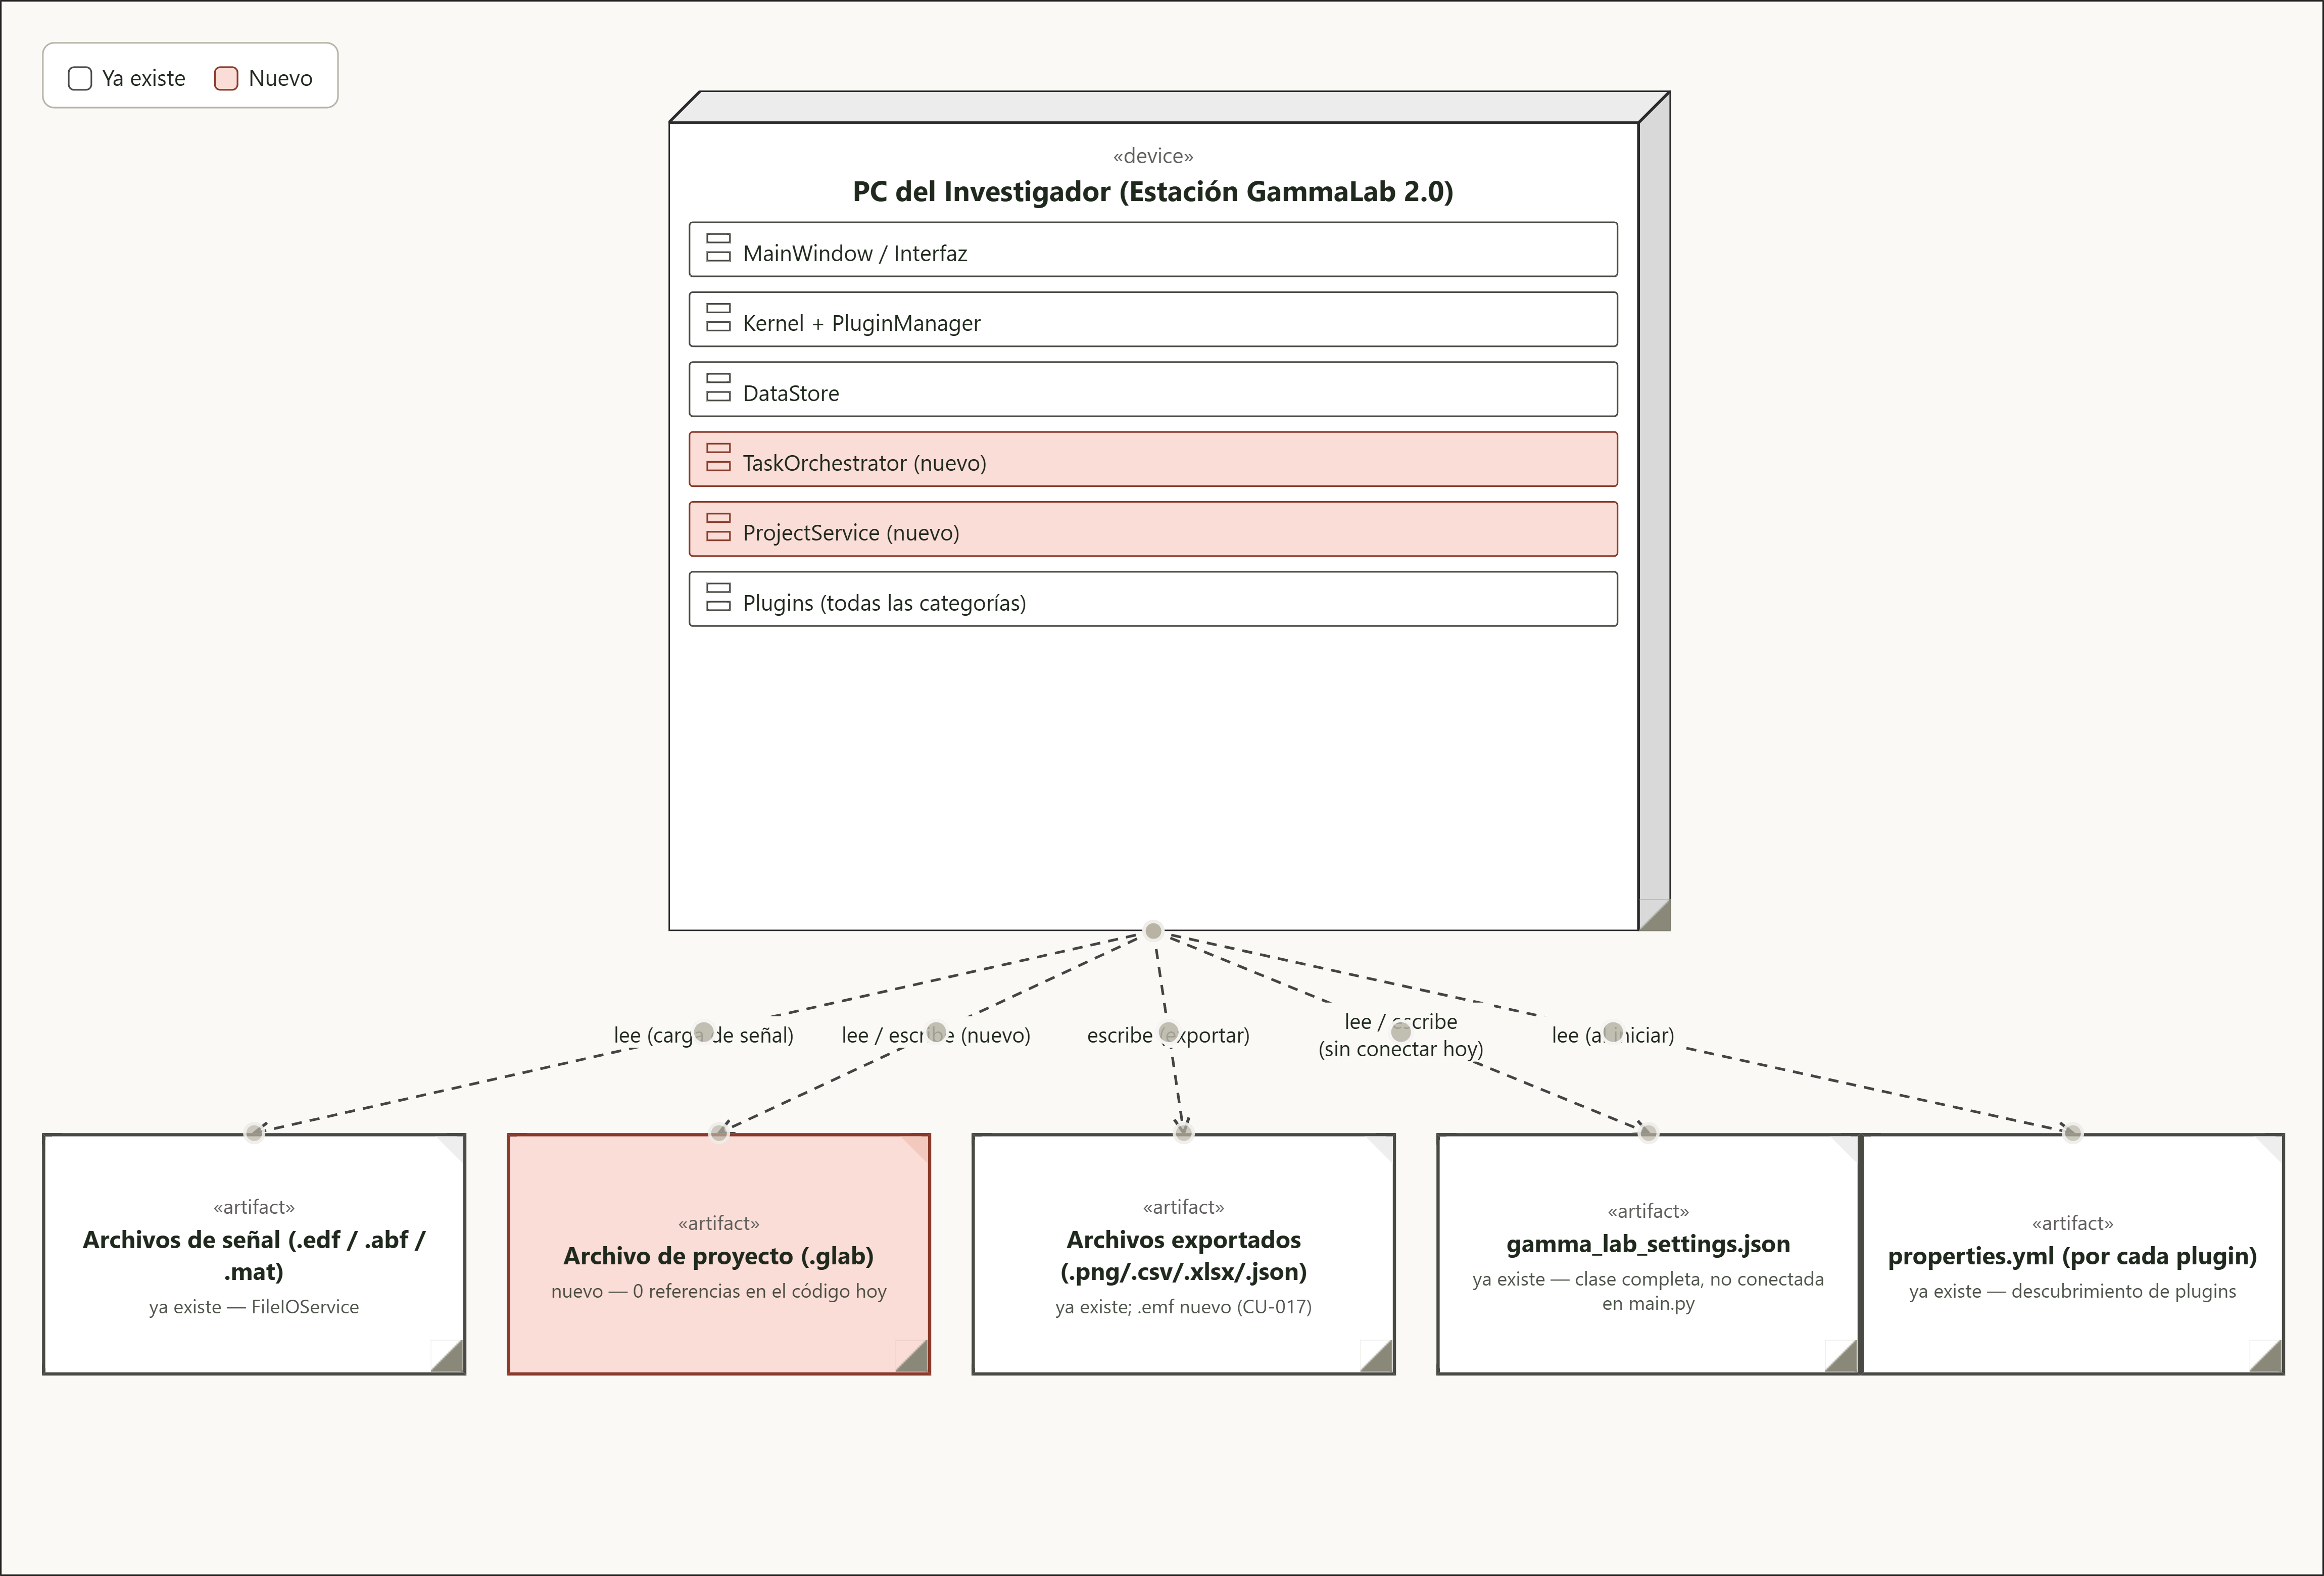
\includegraphics[width=0.85\linewidth]{diagrama_despliegue_sistema_completo.png}
    \caption{Vista f\'isica de GammaLab 2.0: estaci\'on \'unica de escritorio y su superficie de entrada/salida.}
    \label{fig:sdd_vista_fisica}
\end{figure}

La Figura~\ref{fig:sdd_vista_fisica} presenta la distribuci\'on f\'isica de los componentes del sistema en el entorno objetivo de ejecuci\'on. A continuaci\'on se describen los elementos principales:

\begin{itemize}
    \item \textbf{\guillemotleft device\guillemotright\ PC}: estaci\'on de trabajo del investigador donde se despliega y ejecuta el sistema completo; no existe arquitectura cliente-servidor.
    \item \textbf{\guillemotleft OS\guillemotright\ Windows 10/11}: sistema operativo base; versi\'on m\'inima Windows~10 de 64 bits.
    \item \textbf{\guillemotleft executionEnvironment\guillemotright\ Python Runtime 3.11}: entorno de ejecuci\'on que sostiene la aplicaci\'on y sus librer\'ias; versi\'on m\'inima 3.11.x.
    \item \textbf{\guillemotleft artifact\guillemotright\ GammaLab.exe}: ejecutable principal, generado con PyInstaller, que inicia la aplicaci\'on y coordina la carga de todos los componentes.
    \item \textbf{\guillemotleft artifact\guillemotright\ Plugins (*.py)}: archivos de plugin cargados din\'amicamente por el Kernel durante la ejecuci\'on.
    \item \textbf{\guillemotleft artifact\guillemotright\ Archivos de se\~nal} (\texttt{.edf}/\texttt{.abf}/\texttt{.mat}): le\'idos por \texttt{FileIOService}.
    \item \textbf{\guillemotleft artifact\guillemotright\ Archivo de proyecto} (\texttt{.glab}): generado y le\'ido por \texttt{ProjectService}.
    \item \textbf{\guillemotleft artifact\guillemotright\ gamma\_\allowbreak lab\_\allowbreak settings.\allowbreak json}: persistencia de configuraci\'on gestionada por \texttt{Settings\-Service}.
    \item \textbf{\guillemotleft artifact\guillemotright\ properties.yml} (por cada plugin): sostiene el descubrimiento autom\'atico de plugins.
\end{itemize}

\subsubsection{Relaciones}

\begin{itemize}
    \item La relaci\'on \textit{loads} indica que el ejecutable principal carga y ejecuta los archivos de plugin durante el tiempo de ejecuci\'on.
    \item La relaci\'on \textit{uses} especifica que el ejecutable principal utiliza los servicios y librer\'ias desplegados dentro del mismo entorno de ejecuci\'on.
\end{itemize}

\subsubsection{Versiones de las librer\'ias}

Las versiones ancladas para las librer\'ias utilizadas, tal como se fijan en \texttt{requirements.txt}, son las siguientes:

\begin{itemize}
    \item \textbf{PyQt5} = Versi\'on 5.15.11 (\texttt{PyQt5-Qt5} 5.15.2)
    \item \textbf{ScientificLibs}
    \begin{itemize}
        \item NumPy = Versi\'on 2.3.4
        \item Pandas = Versi\'on 2.3.3
        \item SciPy = Versi\'on 1.16.2
        \item PyWavelets = Versi\'on 1.9.0
    \end{itemize}
    \item \textbf{VTK} = Versi\'on 9.5.2
    \item \textbf{EEGReaders}
    \begin{itemize}
        \item pyABF = Versi\'on 2.3.8
        \item pyEDFlib = Versi\'on 0.1.42
    \end{itemize}
    \item \textbf{Otras}
    \begin{itemize}
        \item h5py = Versi\'on 3.15.1
        \item PyYAML = Versi\'on 6.0.3
        \item PyQtWebEngine = Versi\'on 5.15.7
    \end{itemize}
\end{itemize}

\subsection{Vista de Procesos}
\subsubsection{Prop\'osito}

La vista de procesos describe el comportamiento din\'amico del sistema completo como un \'unico flujo maestro de sesi\'on, construido a partir de las cadenas de precondici\'on entre los casos de uso del sistema (p.\,ej.\ generar trials exige una se\~nal previamente cargada).

\begin{figure}[htbp]
    \centering
    \includegraphics[width=0.95\linewidth]{diagrama_actividad_sistema_completo.png}
    \caption{Flujo maestro de sesi\'on de GammaLab 2.0, con carriles Investigador/Sistema.}
    \label{fig:sdd_vista_procesos}
\end{figure}

El flujo de la Figura~\ref{fig:sdd_vista_procesos} se organiza en las siguientes etapas:

\begin{enumerate}
    \item \textbf{Inicio.} El sistema registra los servicios del n\'ucleo, incluido el \texttt{Task\-Orchestrator}, y descubre los plugins disponibles a partir de sus archivos \texttt{properties.yml}.
    \item \textbf{Apertura o carga.} El investigador abre un archivo de proyecto \texttt{.glab} o carga una se\~nal desde la pantalla \textit{Home}; la se\~nal activa se publica en \texttt{DataStore}.
    \item \textbf{Preprocesamiento.} Generaci\'on y edici\'on de trials, selecci\'on de trials, remoci\'on de artefactos, filtrado y ajuste de la frecuencia de muestreo.
    \item \textbf{An\'alisis.} C\'alculo de acoplamiento fase-amplitud (PAC) de un canal o cruzado entre canales, transformada Wavelet y promedio de trials.
    \item \textbf{Orquestaci\'on.} Todo c\'omputo pesado se despacha al \texttt{Task\-Orchestrator} del n\'ucleo, que lo ejecuta fuera del hilo de interfaz y permite su cancelaci\'on en cualquier momento.
    \item \textbf{Visualizaci\'on.} Interacci\'on visual con el resultado, con submuestreo autom\'atico cuando la se\~nal es de gran tama\~no.
    \item \textbf{Iteraci\'on o cierre.} El investigador retorna al preprocesamiento para continuar el an\'alisis, o exporta y guarda el proyecto mediante \texttt{ProjectService} antes de cerrar la sesi\'on.
\end{enumerate}

La navegaci\'on entre secciones, la limpieza de formularios y la ayuda contextual mediante \texttt{Tooltip\-Helper} son transversales a toda la sesi\'on: no ocupan un lugar fijo en la secuencia y se documentan como notas adjuntas al diagrama en vez de forzarse dentro del flujo principal.

\section{Diseño Detallado}

\subsection{Objetivo de la sección}

Esta sección desarrolla el detalle técnico de GammaLab 2.0: la estructura de clases de cada componente, el comportamiento observable del sistema a nivel de interacción entre objetos, los modelos de datos persistidos en memoria y las relaciones entre entidades. Complementa la Sección 2 (Arquitectura), que describe el sistema a nivel de componentes y procesos, con el nivel de detalle necesario para la implementación.

\subsection{Estructura del Sistema}

\subsubsection{Propósito}

El propósito de esta sección es documentar la estructura de clases de cada componente del sistema, sirviendo como guía para su implementación.

\subsubsection{Organización general}

El código fuente de GammaLab 2.0 sigue la misma organización por responsabilidades presentada en la Vista Lógica (Sección 2.1): cada componente concentra un conjunto cohesivo de clases y se comunica con los demás mediante los servicios registrados en el \texttt{Kernel}. El diagrama de clases completo del sistema se presenta en la Figura~\ref{fig:sdd_vista_logica} (Sección 2.1); a continuación se detalla cada componente por separado.

\subsubsection{Descripción de clases por componentes}

\begin{enumerate}

\item \textbf{Componente: ApplicationCore}

El componente \textbf{ApplicationCore} concentra el núcleo del sistema: el registro de plugins y servicios, el contrato de extensión (\texttt{IPlugin}) y las utilidades compartidas por el resto de la aplicación.

\begin{figure}[htbp]
    \centering
    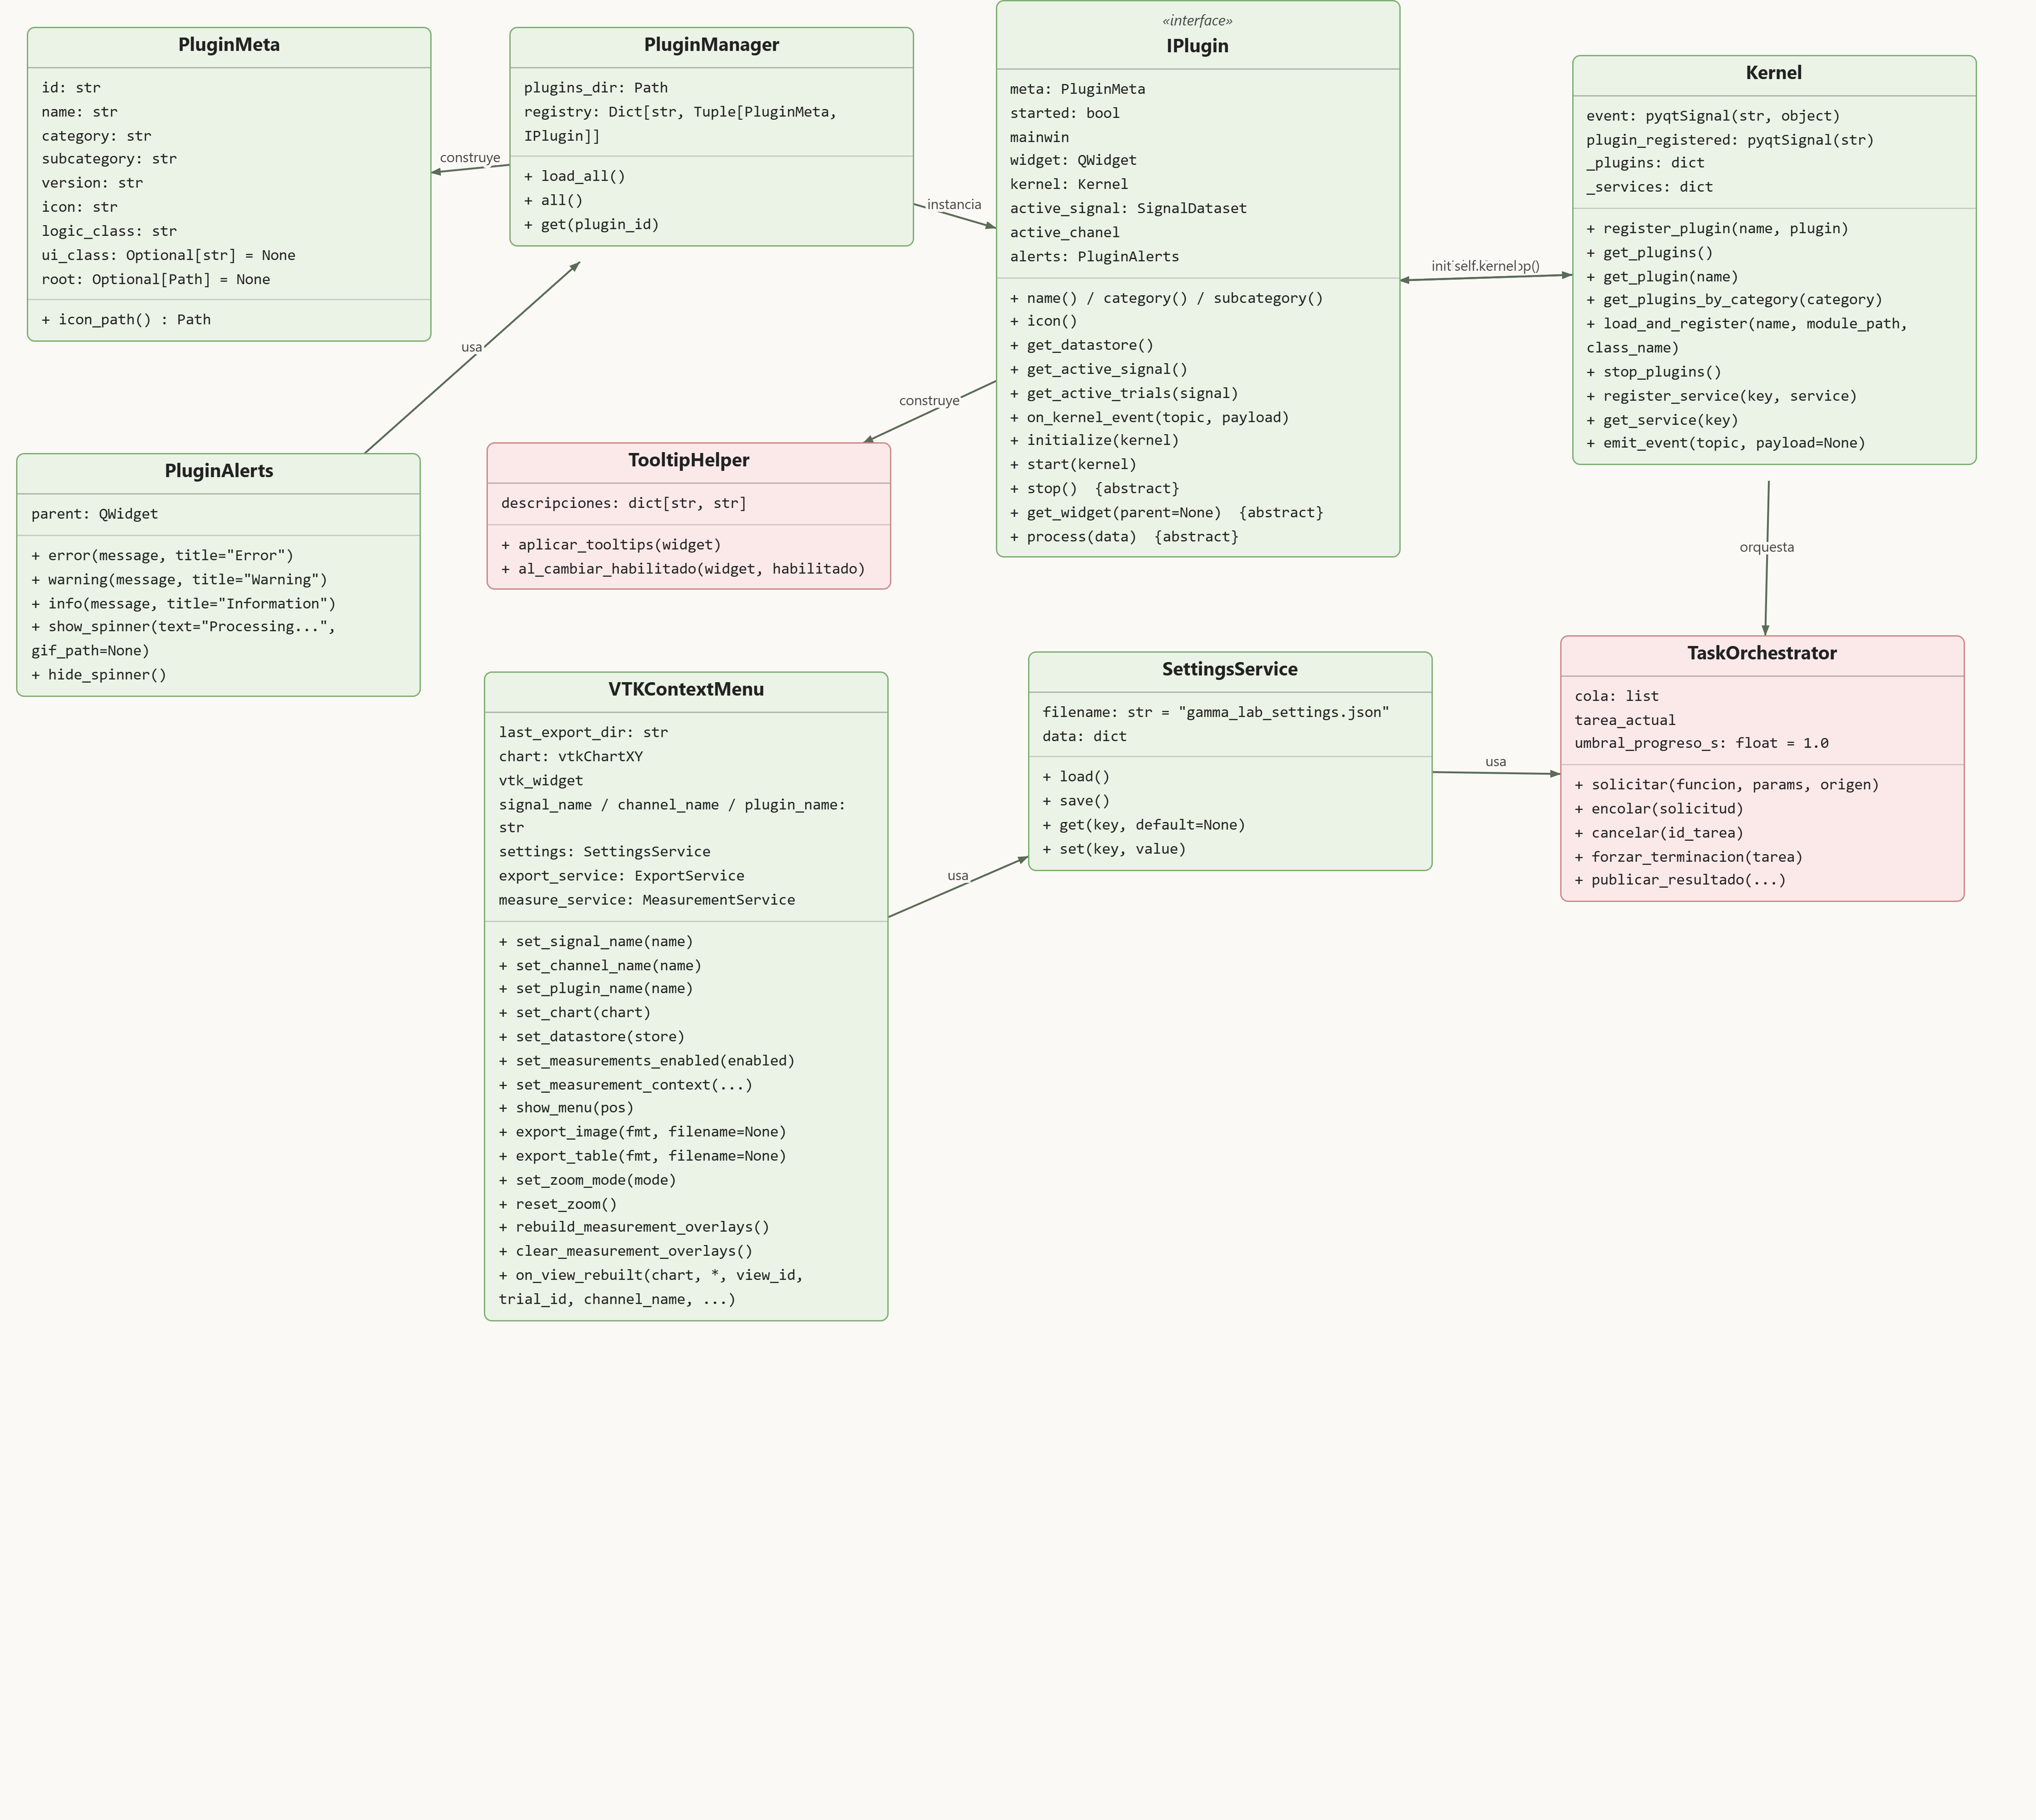
\includegraphics[width=0.95\linewidth]{diagramas_html/application_core.png}
    \caption{Diagrama de clases --- componente ApplicationCore}
    \label{fig:sdd_dc_appcore}
\end{figure}

Las clases del componente \textit{ApplicationCore} son las siguientes:

\textbf{PluginMeta} Metadatos y configuración de un plugin descubierto por el sistema.
\begin{itemize}
    \item \textbf{Atributos principales:} \texttt{id}, \texttt{name}, \texttt{category}, \texttt{subcategory}, \texttt{version}, \texttt{icon}: \texttt{str}; \texttt{logic\_\allowbreak class}, \texttt{ui\_\allowbreak class: Optional[str] = None}; \texttt{root: Optional[Path] = None}.
    \item \textbf{Métodos principales:} \texttt{icon\_\allowbreak path(): Path}.
\end{itemize}

\textbf{PluginManager} Gestor central de descubrimiento y registro de plugins a partir de sus archivos \texttt{properties.yml}.
\begin{itemize}
    \item \textbf{Atributos principales:} \texttt{plugins\_\allowbreak dir: Path}; \texttt{registry: Dict[str, Tuple[PluginMeta, IPlugin]]}.
    \item \textbf{Métodos principales:} \texttt{load\_\allowbreak all()}, \texttt{all()}, \texttt{get(plugin\_\allowbreak id)}.
\end{itemize}

\textbf{IPlugin} («interface») Contrato que toda extensión del sistema implementa.
\begin{itemize}
    \item \textbf{Atributos principales:} \texttt{meta: PluginMeta}; \texttt{started: bool}; \texttt{mainwin}; \texttt{widget: QWidget}; \texttt{kernel: Kernel}; \texttt{active\_\allowbreak signal: SignalDataset}; \texttt{active\_\allowbreak chanel}; \texttt{alerts: PluginAlerts}.
    \item \textbf{Métodos principales:} \texttt{name()}/\allowbreak\texttt{category()}/\allowbreak\texttt{subcategory()}, \texttt{icon()}, \texttt{get\_\allowbreak datastore()}, \texttt{get\_\allowbreak active\_\allowbreak signal()}, \texttt{get\_\allowbreak active\_\allowbreak trials(signal)}, \texttt{on\_\allowbreak kernel\_\allowbreak event(topic, payload)}, \texttt{initialize(kernel)}, \texttt{start(kernel)}, \texttt{stop()} \{abstracto\}, \texttt{get\_\allowbreak widget(parent=None)} \{abstracto\}, \texttt{process(data)} \{abstracto\}.
\end{itemize}

\textbf{Kernel} Núcleo central de la aplicación; implementa el patrón microkernel con inversión de control sobre servicios y plugins.
\begin{itemize}
    \item \textbf{Atributos principales:} \texttt{event: pyqtSignal(str, object)}; \texttt{plugin\_\allowbreak registered: pyqtSignal(str)}; \texttt{\_\allowbreak plugins: dict}; \texttt{\_\allowbreak services: dict}.
    \item \textbf{Métodos principales:} \texttt{register\_\allowbreak plugin(name, plugin)}, \texttt{get\_\allowbreak plugins()}, \texttt{get\_\allowbreak plugin(name)}, \texttt{get\_\allowbreak plugins\_\allowbreak by\_\allowbreak category(category)}, \texttt{load\_\allowbreak and\_\allowbreak register(name, module\_\allowbreak path, class\_\allowbreak name)}, \texttt{stop\_\allowbreak plugins()}, \texttt{register\_\allowbreak service(key, service)}, \texttt{get\_\allowbreak service(key)}, \texttt{emit\_\allowbreak event(topic, payload=None)}.
\end{itemize}

\textbf{SettingsService} Servicio de configuración general del sistema y preferencias del usuario.
\begin{itemize}
    \item \textbf{Atributos principales:} \texttt{filename: str = "gamma\_\allowbreak lab\_\allowbreak settings.json"}; \texttt{data: dict}.
    \item \textbf{Métodos principales:} \texttt{load()}, \texttt{save()}, \texttt{get(key, default=None)}, \texttt{set(key, value)}.
\end{itemize}

\textbf{VTKContextMenu} Menú contextual general para vistas basadas en VTK; delega en \texttt{ExportService} y \texttt{MeasurementService} (ver esos componentes).
\begin{itemize}
    \item \textbf{Atributos principales:} \texttt{last\_\allowbreak export\_\allowbreak dir: str}; \texttt{chart: vtkChartXY}; \texttt{vtk\_\allowbreak widget}; \texttt{signal\_\allowbreak name}/\allowbreak\texttt{channel\_\allowbreak name}/\allowbreak\texttt{plugin\_\allowbreak name: str}; \texttt{settings: SettingsService}; \texttt{export\_\allowbreak service: ExportService}; \texttt{measure\_\allowbreak service: MeasurementService}.
    \item \textbf{Métodos principales:} \texttt{set\_\allowbreak signal\_\allowbreak name(name)}, \texttt{set\_\allowbreak channel\_\allowbreak name(name)}, \texttt{set\_\allowbreak plugin\_\allowbreak name(name)}, \texttt{set\_\allowbreak chart(chart)}, \texttt{set\_\allowbreak datastore(store)}, \texttt{set\_\allowbreak measurements\_\allowbreak enabled(enabled)}, \texttt{set\_\allowbreak measurement\_\allowbreak context(\ldots)}, \texttt{show\_\allowbreak menu(pos)}, \texttt{export\_\allowbreak image(fmt, filename=None)}, \texttt{export\_\allowbreak table(fmt, filename=None)}, \texttt{set\_\allowbreak zoom\_\allowbreak mode(mode)}, \texttt{reset\_\allowbreak zoom()}, \texttt{rebuild\_\allowbreak measurement\_\allowbreak overlays()}, \texttt{clear\_\allowbreak measurement\_\allowbreak overlays()}, \texttt{on\_\allowbreak view\_\allowbreak rebuilt(chart, *, view\_\allowbreak id, trial\_\allowbreak id, channel\_\allowbreak name, \ldots)}.
\end{itemize}

\textbf{PluginAlerts} Sistema de notificaciones y alertas reutilizado por los servicios y los plugins.
\begin{itemize}
    \item \textbf{Atributos principales:} \texttt{parent: QWidget}.
    \item \textbf{Métodos principales:} \texttt{error(message, title="Error")}, \texttt{warning(message, title="Warning")}, \texttt{info(message, title="Information")}, \texttt{show\_\allowbreak spinner(text="Processing...", gif\_\allowbreak path=None)}, \texttt{hide\_\allowbreak spinner()}.
\end{itemize}

\textbf{TaskOrchestrator} Centraliza la ejecución de cómputo pesado (PAC, Wavelet, PSD) fuera del hilo de interfaz, con soporte de cancelación.
\begin{itemize}
    \item \textbf{Atributos principales:} \texttt{cola: list}; \texttt{tarea\_\allowbreak actual}; \texttt{umbral\_\allowbreak progreso\_\allowbreak s: float = 1.0}.
    \item \textbf{Métodos principales:} \texttt{solicitar(funcion, params, origen)}, \texttt{encolar(solicitud)}, \texttt{cancelar(id\_\allowbreak tarea)}, \texttt{forzar\_\allowbreak terminacion(tarea)}, \texttt{publicar\_\allowbreak resultado(\ldots)}.
\end{itemize}

\textbf{TooltipHelper} Ayuda contextual mediante tooltips dinámicos sobre los controles de la interfaz.
\begin{itemize}
    \item \textbf{Atributos principales:} \texttt{descripciones: dict[str, str]}.
    \item \textbf{Métodos principales:} \texttt{aplicar\_\allowbreak tooltips(widget)}, \texttt{al\_\allowbreak cambiar\_\allowbreak habilitado(widget, habilitado)}.
\end{itemize}

\texttt{TaskOrchestrator} y \texttt{TooltipHelper} son clases nuevas: no existen aún en el código de GammaLab 2.0. Las demás clases del componente sí están implementadas, con una salvedad: \texttt{SettingsService} está completa pero no se registra en \texttt{main.py} hoy, por lo que ningún plugin la consume actualmente a través del Kernel.

\item \textbf{Componente: MainUI}

El componente \textbf{MainUI} provee al núcleo la interfaz principal de la aplicación.

\begin{figure}[htbp]
    \centering
    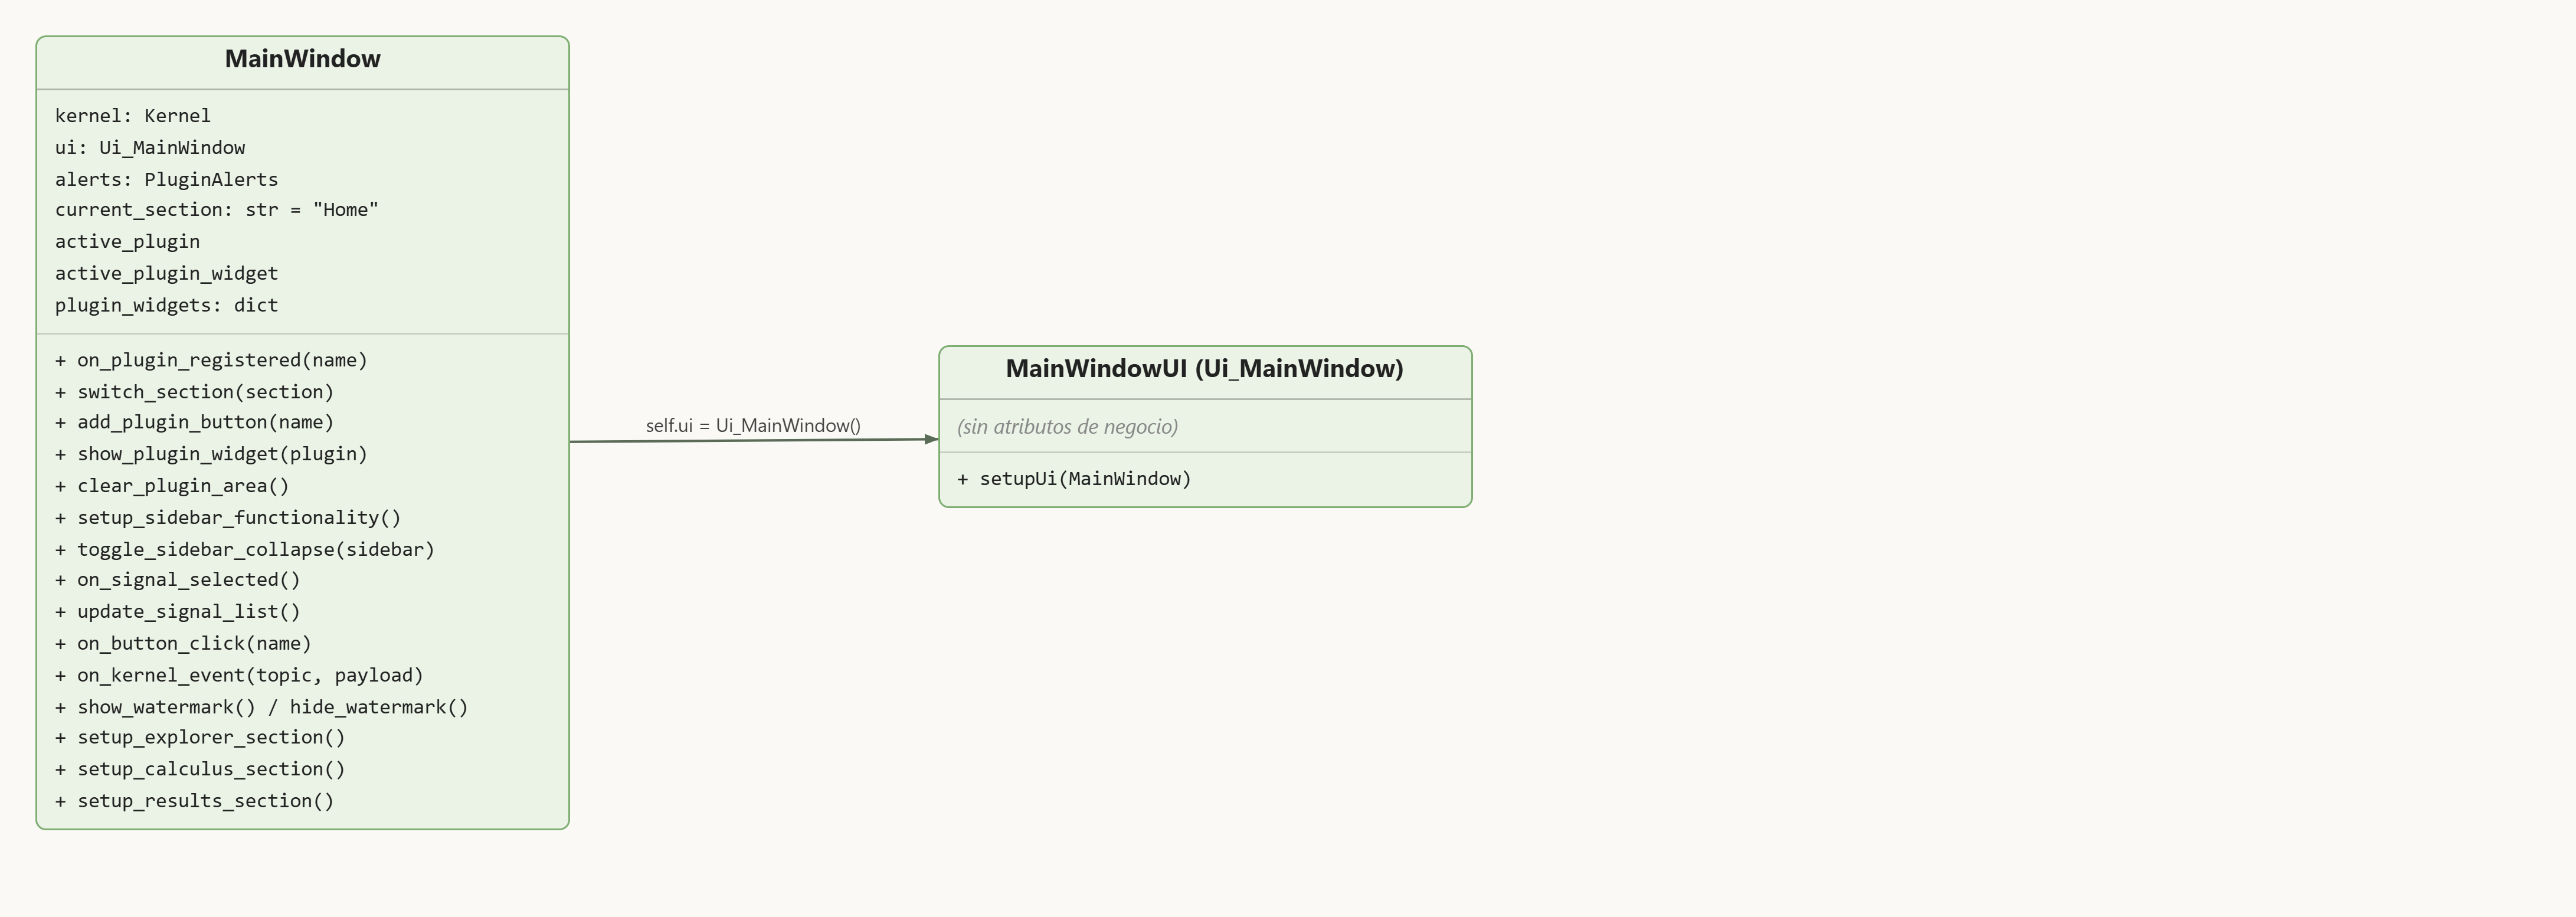
\includegraphics[width=0.8\linewidth]{diagramas_html/main_ui.png}
    \caption{Diagrama de clases --- componente MainUI}
    \label{fig:sdd_dc_mainui}
\end{figure}

\textbf{MainWindow} Ventana principal de la aplicación; se registra a sí misma como servicio del Kernel ("MainWindow") y coordina la interfaz con los plugins.
\begin{itemize}
    \item \textbf{Atributos principales:} \texttt{kernel: Kernel}; \texttt{ui: Ui\_\allowbreak MainWindow}; \texttt{alerts: PluginAlerts}; \texttt{current\_\allowbreak section: str = "Home"}; \texttt{active\_\allowbreak plugin}; \texttt{active\_\allowbreak plugin\_\allowbreak widget}; \texttt{plugin\_\allowbreak widgets: dict}.
    \item \textbf{Métodos principales:} \texttt{on\_\allowbreak plugin\_\allowbreak registered(name)}, \texttt{switch\_\allowbreak section(section)}, \texttt{add\_\allowbreak plugin\_\allowbreak button(name)}, \texttt{show\_\allowbreak plugin\_\allowbreak widget(plugin)}, \texttt{clear\_\allowbreak plugin\_\allowbreak area()}, \texttt{setup\_\allowbreak sidebar\_\allowbreak functionality()}, \texttt{toggle\_\allowbreak sidebar\_\allowbreak collapse(sidebar)}, \texttt{on\_\allowbreak signal\_\allowbreak selected()}, \texttt{update\_\allowbreak signal\_\allowbreak list()}, \texttt{on\_\allowbreak button\_\allowbreak click(name)}, \texttt{on\_\allowbreak kernel\_\allowbreak event(topic, payload)}, \texttt{show\_\allowbreak watermark()}/\allowbreak\texttt{hide\_\allowbreak watermark()}, \texttt{setup\_\allowbreak explorer\_\allowbreak section()}, \texttt{setup\_\allowbreak calculus\_\allowbreak section()}, \texttt{setup\_\allowbreak results\_\allowbreak section()}.
\end{itemize}

\textbf{MainWindowUI (\texttt{Ui\_\allowbreak MainWindow})} Construcción visual de la ventana principal, sin lógica de negocio propia.
\begin{itemize}
    \item \textbf{Métodos principales:} \texttt{setupUi(MainWindow)}.
\end{itemize}

\texttt{MainWindow} consulta el servicio \texttt{DataStore} (vía \texttt{kernel.get\_\allowbreak service("DataStore")}) para poblar la lista de señales, e invoca \texttt{get\_\allowbreak widget()}, \texttt{start()}, \texttt{process()} y \texttt{stop()} de cada \texttt{IPlugin} registrado.

\item \textbf{Componente: Plugins}

El componente \textbf{Plugins} es el punto de extensión del sistema: toda funcionalidad de entrada/salida, preprocesamiento y análisis se implementa como un plugin que respeta el contrato \texttt{IPlugin}.

\begin{figure}[htbp]
    \centering
    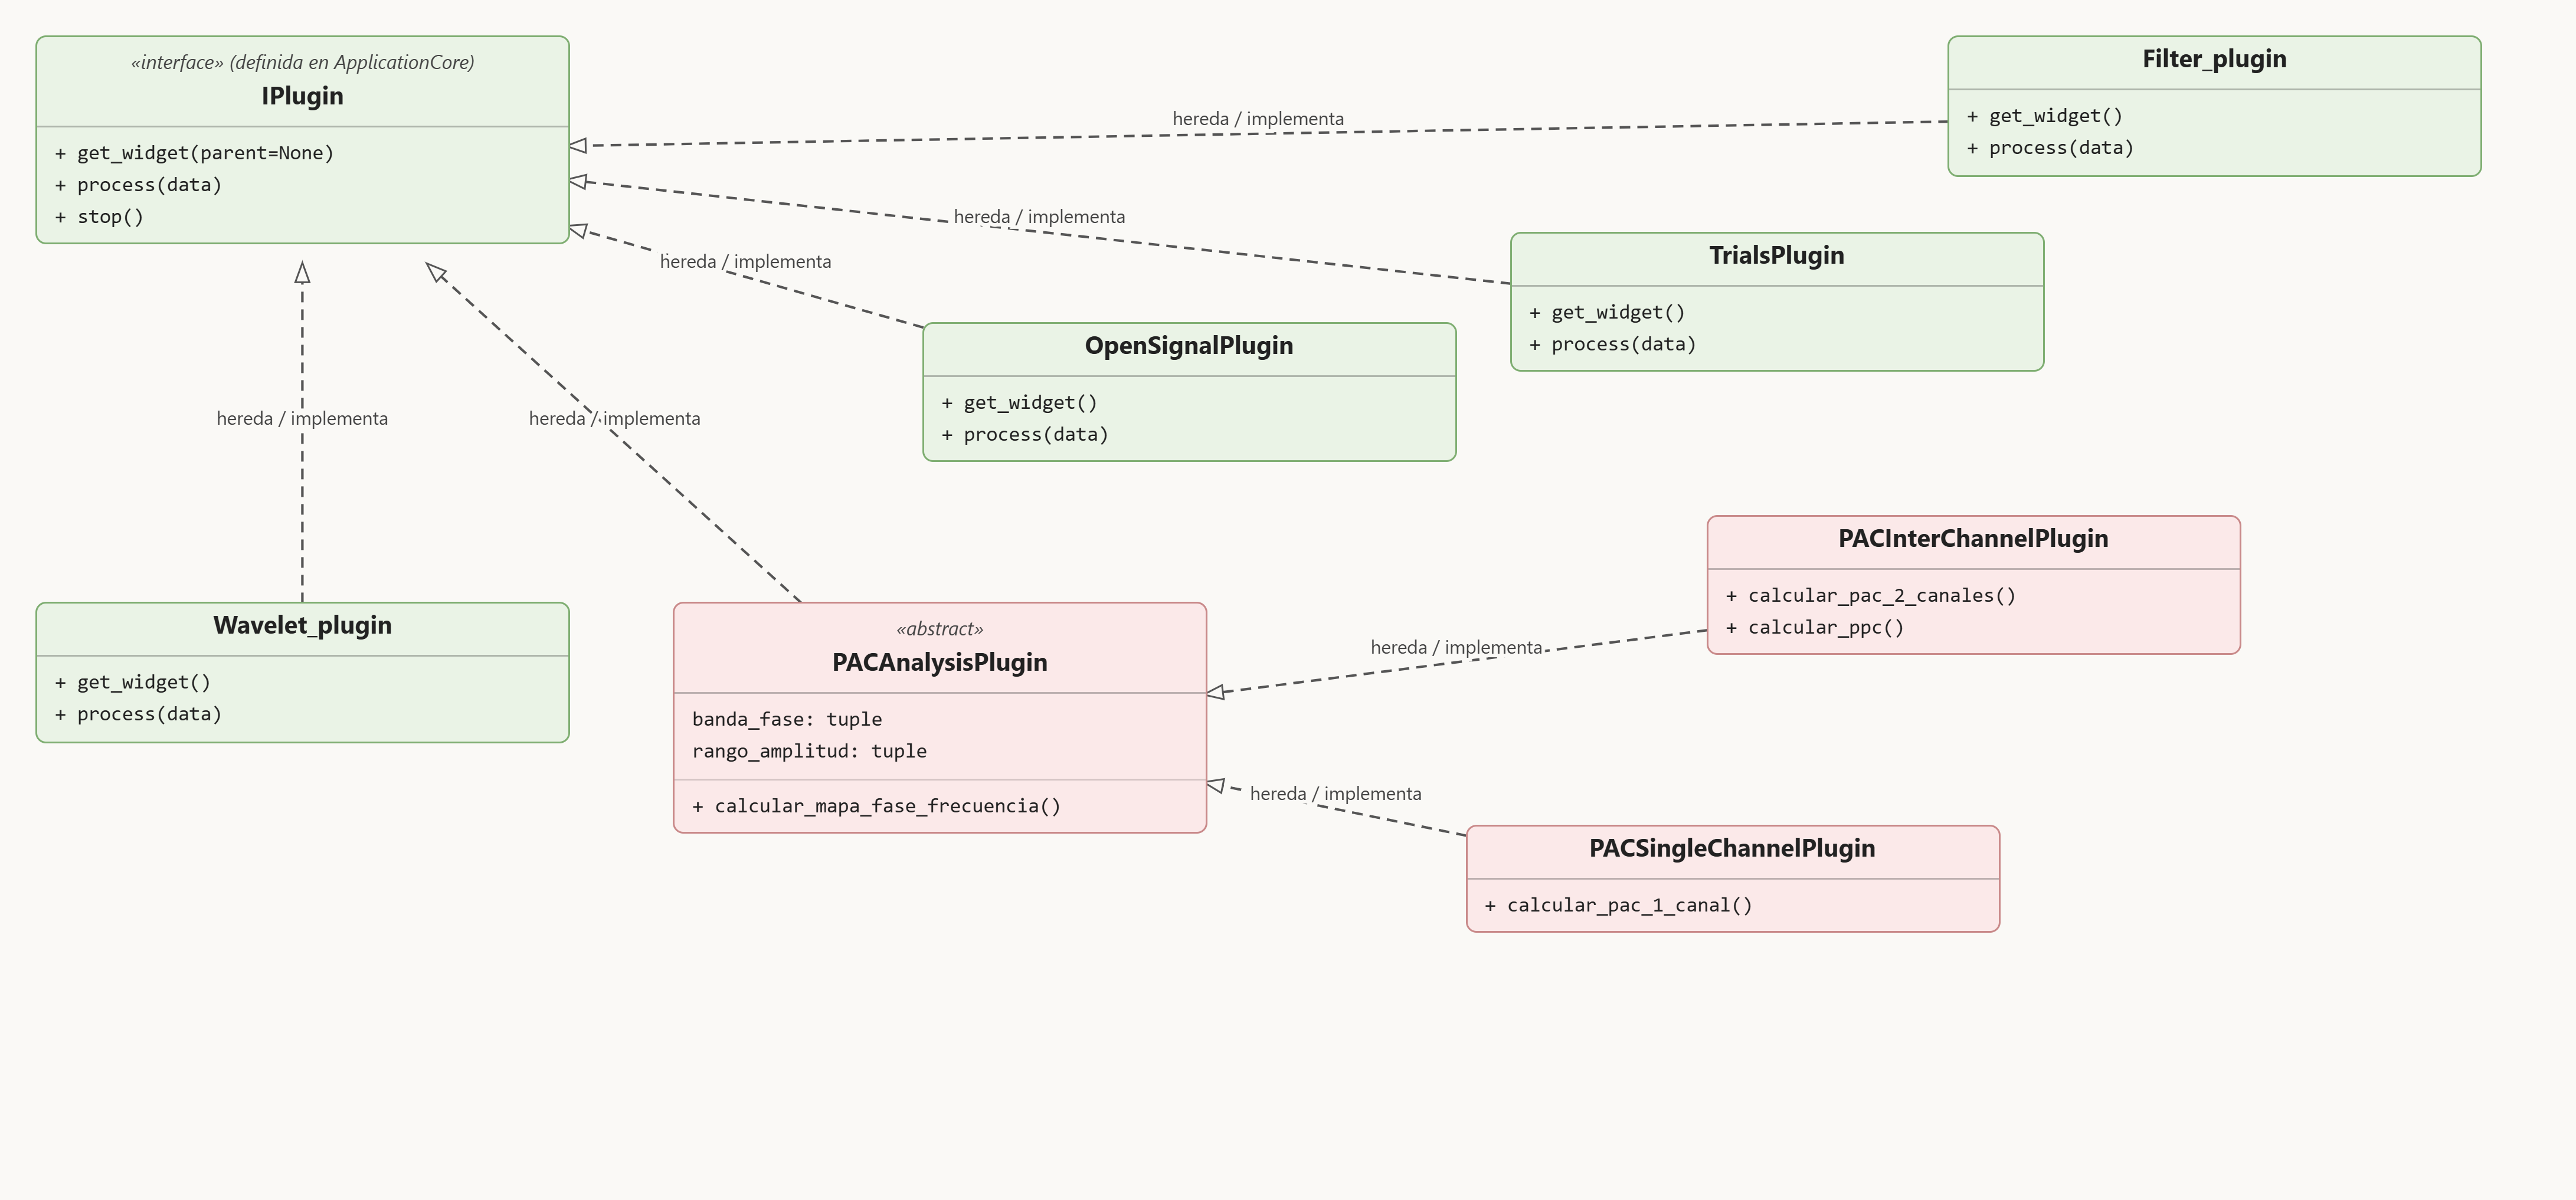
\includegraphics[width=0.95\linewidth]{diagramas_html/plugins.png}
    \caption{Diagrama de clases --- componente Plugins}
    \label{fig:sdd_dc_plugins}
\end{figure}

\textbf{OpenSignalPlugin}, \textbf{TrialsPlugin}, \textbf{Filter\_\allowbreak plugin} y \textbf{Wavelet\_\allowbreak plugin} son cuatro ejemplos representativos de los plugins ya existentes en el sistema (el repositorio incluye 16 en total: FFT, PSD, Average, ERP, Amplitude, Slope, ArtifactRemove, FAQ, entre otros). Todos implementan \texttt{get\_\allowbreak widget()} y \texttt{process(data)} de \texttt{IPlugin}, y son descubiertos por \texttt{PluginManager} a partir de su \texttt{properties.yml}; el nombre de la clase declarado ahí (\texttt{logic\_\allowbreak class}) no siempre coincide con el nombre de la carpeta del plugin.

\textbf{PACAnalysisPlugin} («abstract», nuevo) Base común de los plugins de acoplamiento fase-amplitud (\textit{Phase-Amplitude Coupling}).
\begin{itemize}
    \item \textbf{Atributos principales:} \texttt{banda\_\allowbreak fase: tuple}; \texttt{rango\_\allowbreak amplitud: tuple}.
    \item \textbf{Métodos principales:} \texttt{calcular\_\allowbreak mapa\_\allowbreak fase\_\allowbreak frecuencia()}.
\end{itemize}

\textbf{PACSingleChannelPlugin} (nuevo) Hereda de \texttt{PACAnalysisPlugin}; calcula el PAC de un único canal.
\begin{itemize}
    \item \textbf{Métodos principales:} \texttt{calcular\_\allowbreak pac\_\allowbreak 1\_\allowbreak canal()}.
\end{itemize}

\textbf{PACInterChannelPlugin} (nuevo) Hereda de \texttt{PACAnalysisPlugin}; calcula el PAC cruzado entre dos canales.
\begin{itemize}
    \item \textbf{Métodos principales:} \texttt{calcular\_\allowbreak pac\_\allowbreak 2\_\allowbreak canales()}, \texttt{calcular\_\allowbreak ppc()}.
\end{itemize}

El cómputo pesado de los plugins de análisis (Wavelet, familia PAC) se despacharía al \texttt{TaskOrchestrator} (ver componente ApplicationCore) en vez de bloquear el hilo de interfaz.

\item \textbf{Componente: DataStore}

El componente \textbf{DataStore}, encargado de la persistencia en memoria, provee un servicio de almacenamiento de tipo clave-valor y define los modelos de datos centrales del sistema.

\begin{figure}[htbp]
    \centering
    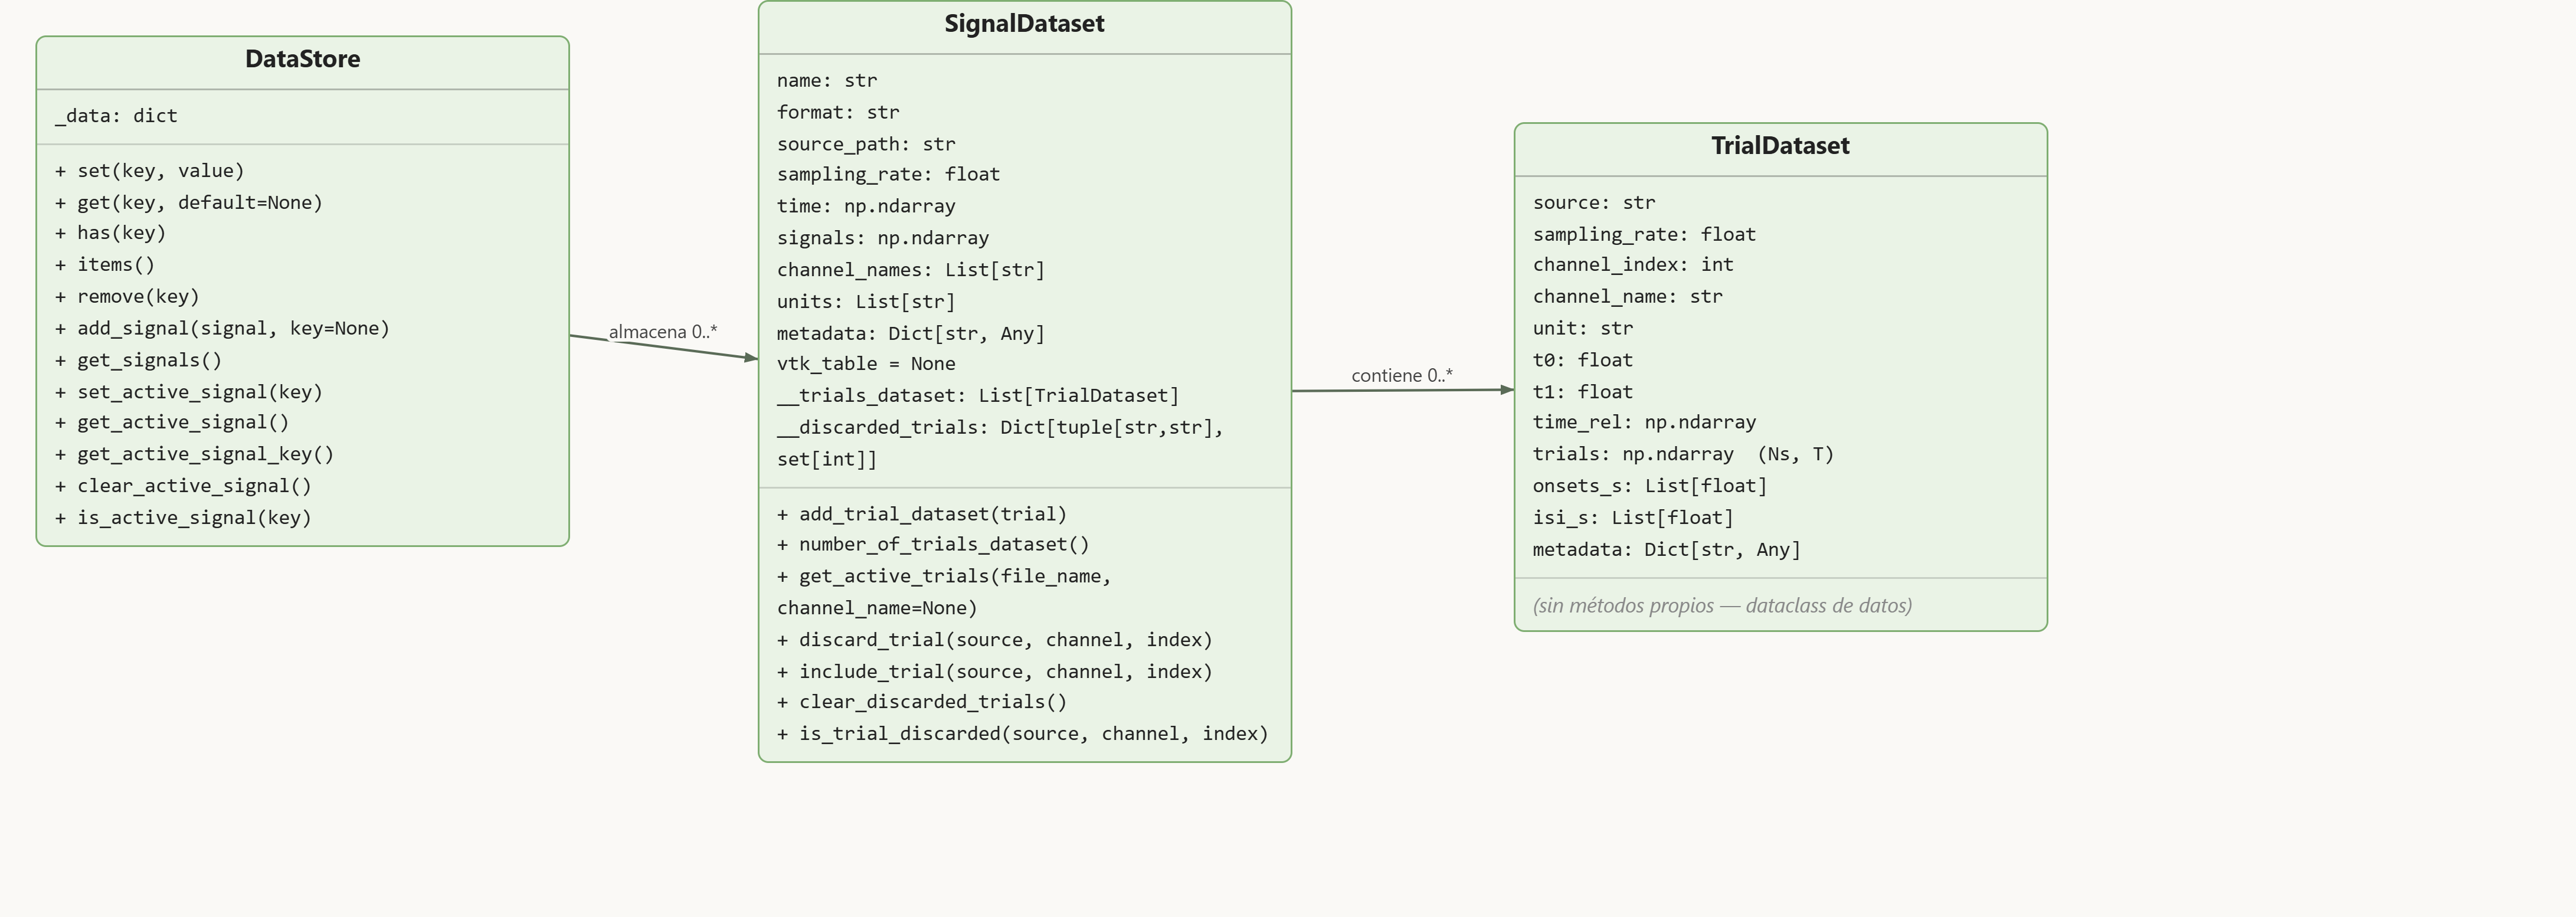
\includegraphics[width=0.95\linewidth]{diagramas_html/data_store.png}
    \caption{Diagrama de clases --- componente DataStore}
    \label{fig:sdd_dc_datastore}
\end{figure}

\textbf{DataStore} Almacén centralizado en memoria de señales, trials y cualquier otro estado indexado por clave.
\begin{itemize}
    \item \textbf{Atributos principales:} \texttt{\_\allowbreak data: dict}.
    \item \textbf{Métodos principales:} \texttt{set(key, value)}, \texttt{get(key, default=None)}, \texttt{has(key)}, \texttt{items()}, \texttt{remove(key)}, \texttt{add\_\allowbreak signal(signal, key=None)}, \texttt{get\_\allowbreak signals()}, \texttt{set\_\allowbreak active\_\allowbreak signal(key)}, \texttt{get\_\allowbreak active\_\allowbreak signal()}, \texttt{get\_\allowbreak active\_\allowbreak signal\_\allowbreak key()}, \texttt{clear\_\allowbreak active\_\allowbreak signal()}, \texttt{is\_\allowbreak active\_\allowbreak signal(key)}.
\end{itemize}

\textbf{SignalDataset} Conjunto completo de datos de una señal cargada, incluyendo sus trials asociados.
\begin{itemize}
    \item \textbf{Atributos principales:} \texttt{name: str}; \texttt{format: str}; \texttt{source\_\allowbreak path: str}; \texttt{sampling\_\allowbreak rate: float}; \texttt{time: np.ndarray}; \texttt{signals: np.ndarray}; \texttt{channel\_\allowbreak names: List[str]}; \texttt{units: List[str]}; \texttt{metadata: Dict[str, Any]}; \texttt{vtk\_\allowbreak table = None}; \texttt{\_\allowbreak \_\allowbreak trials\_\allowbreak dataset: List[TrialDataset]}; \texttt{\_\allowbreak \_\allowbreak discarded\_\allowbreak trials: Dict[tuple[str,str], set[int]]}.
    \item \textbf{Métodos principales:} \texttt{add\_\allowbreak trial\_\allowbreak dataset(trial)}, \texttt{number\_\allowbreak of\_\allowbreak trials\_\allowbreak dataset()}, \texttt{get\_\allowbreak active\_\allowbreak trials(file\_\allowbreak name, channel\_\allowbreak name=None)}, \texttt{discard\_\allowbreak trial(source, channel, index)}, \texttt{include\_\allowbreak trial(source, channel, index)}, \texttt{clear\_\allowbreak discarded\_\allowbreak trials()}, \texttt{is\_\allowbreak trial\_\allowbreak discarded(source, channel, index)}.
\end{itemize}

\textbf{TrialDataset} Partición (ensayo) de una señal, usada para análisis focalizados.
\begin{itemize}
    \item \textbf{Atributos principales:} \texttt{source: str}; \texttt{sampling\_\allowbreak rate: float}; \texttt{channel\_\allowbreak index: int}; \texttt{channel\_\allowbreak name: str}; \texttt{unit: str}; \texttt{t0}/\allowbreak\texttt{t1: float}; \texttt{time\_\allowbreak rel: np.ndarray}; \texttt{trials: np.ndarray (Ns, T)}; \texttt{onsets\_\allowbreak s: List[float]}; \texttt{isi\_\allowbreak s: List[float]}; \texttt{metadata: Dict[str, Any]}.
    \item \textbf{Métodos principales:} sin métodos propios --- es una estructura de datos consumida por \texttt{SignalDataset}.
\end{itemize}

\texttt{FileIOService} (ver componente FileIO) construye instancias de \texttt{SignalDataset} a partir de archivos externos; \texttt{TaskOrchestrator} y \texttt{ProjectSession} (ver esos componentes) leerían y escribirían en \texttt{DataStore}.

\item \textbf{Componente: FileIO}

El componente \textbf{FileIO} es responsable de la lectura de archivos de señal EEG en múltiples formatos.

\begin{figure}[htbp]
    \centering
    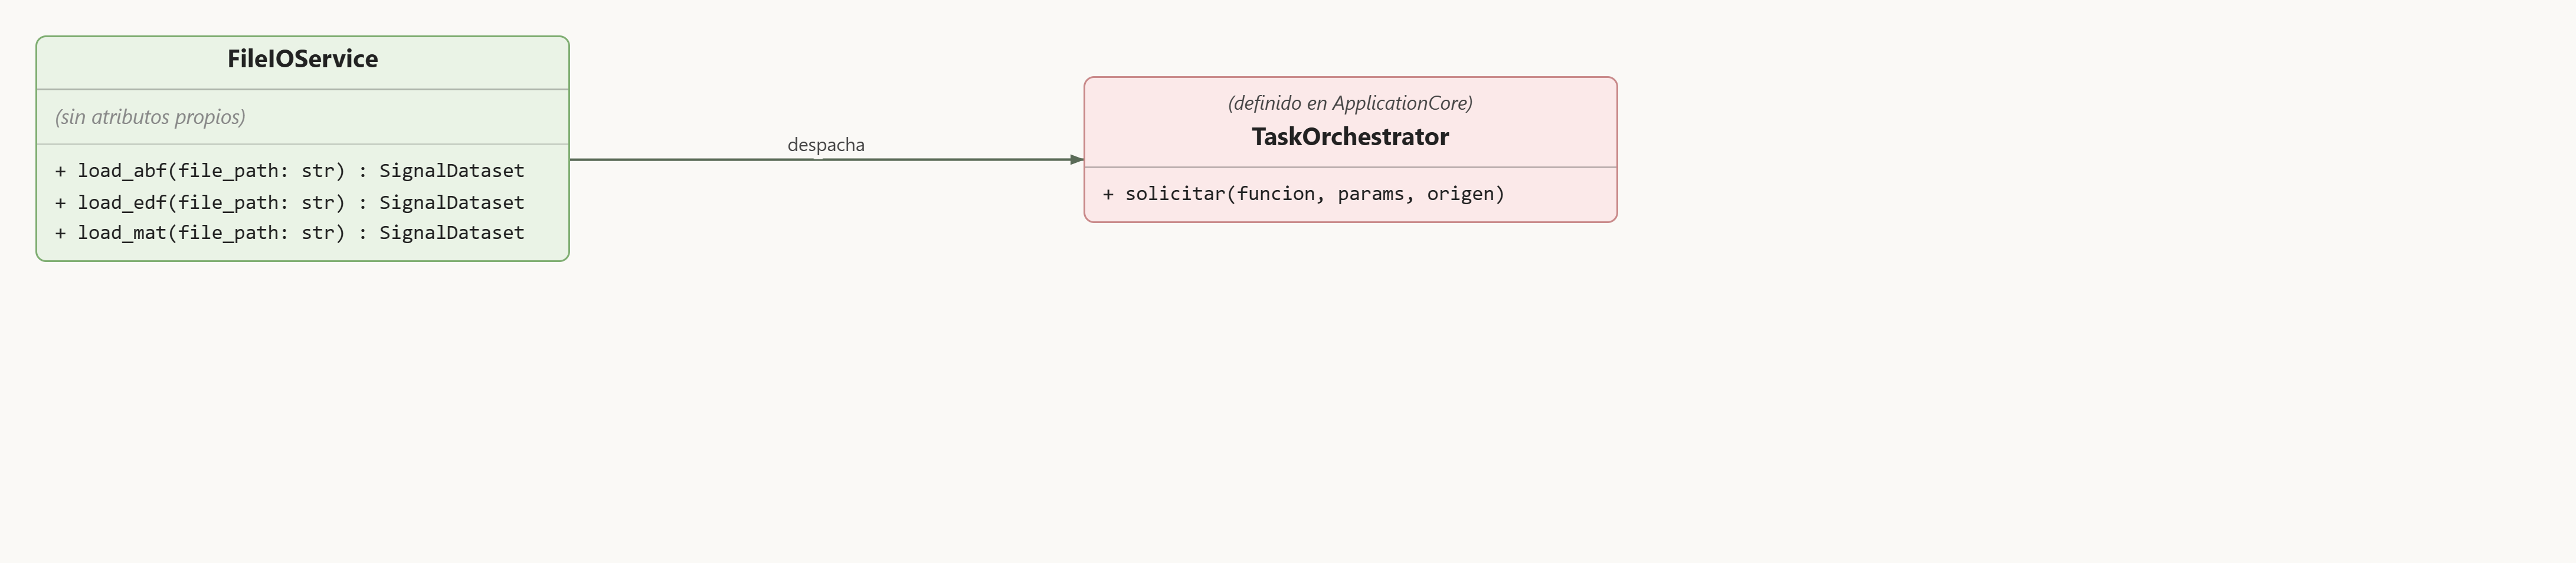
\includegraphics[width=0.7\linewidth]{diagramas_html/file_io.png}
    \caption{Diagrama de clases --- componente FileIO}
    \label{fig:sdd_dc_fileio}
\end{figure}

\textbf{FileIOService} Servicio de lectura de archivos que construye instancias de \texttt{SignalDataset}.
\begin{itemize}
    \item \textbf{Métodos principales:} \texttt{load\_\allowbreak abf(file\_\allowbreak path: str): SignalDataset}, \texttt{load\_\allowbreak edf(file\_\allowbreak path: str): SignalDataset}, \texttt{load\_\allowbreak mat(file\_\allowbreak path: str): SignalDataset}.
\end{itemize}

\texttt{FileIOService} usa las librerías externas \texttt{pyabf}, \texttt{pyedflib}, \texttt{scipy.io.loadmat} y \texttt{h5py}. El Kernel registra el servicio bajo la clave \texttt{"FileIO"} (no \texttt{"FileIOService"}); si \texttt{OpenSignalPlugin} no lo encuentra registrado, crea uno propio y lo registra él mismo. \texttt{load\_\allowbreak mat()} está implementado y funciona correctamente, pero la rama que lo invoca en \texttt{OpenSignalPlugin} está comentada hoy: desde la interfaz solo se pueden cargar archivos \texttt{.abf} y \texttt{.edf}. El SAD (Escenario de Calidad 2) documenta que esta lectura debería despacharse al \texttt{TaskOrchestrator} para no bloquear la interfaz; hoy \texttt{OpenSignalPlugin} llama a \texttt{load\_\allowbreak abf()}/\allowbreak\texttt{load\_\allowbreak edf()} de forma directa y síncrona en el hilo de interfaz, sin que el orquestador intervenga todavía en esta ruta.

\item \textbf{Componente: Export}

El componente \textbf{Export} es responsable de la generación de archivos de salida (imagen y tabla) a partir de las visualizaciones activas.

\begin{figure}[htbp]
    \centering
    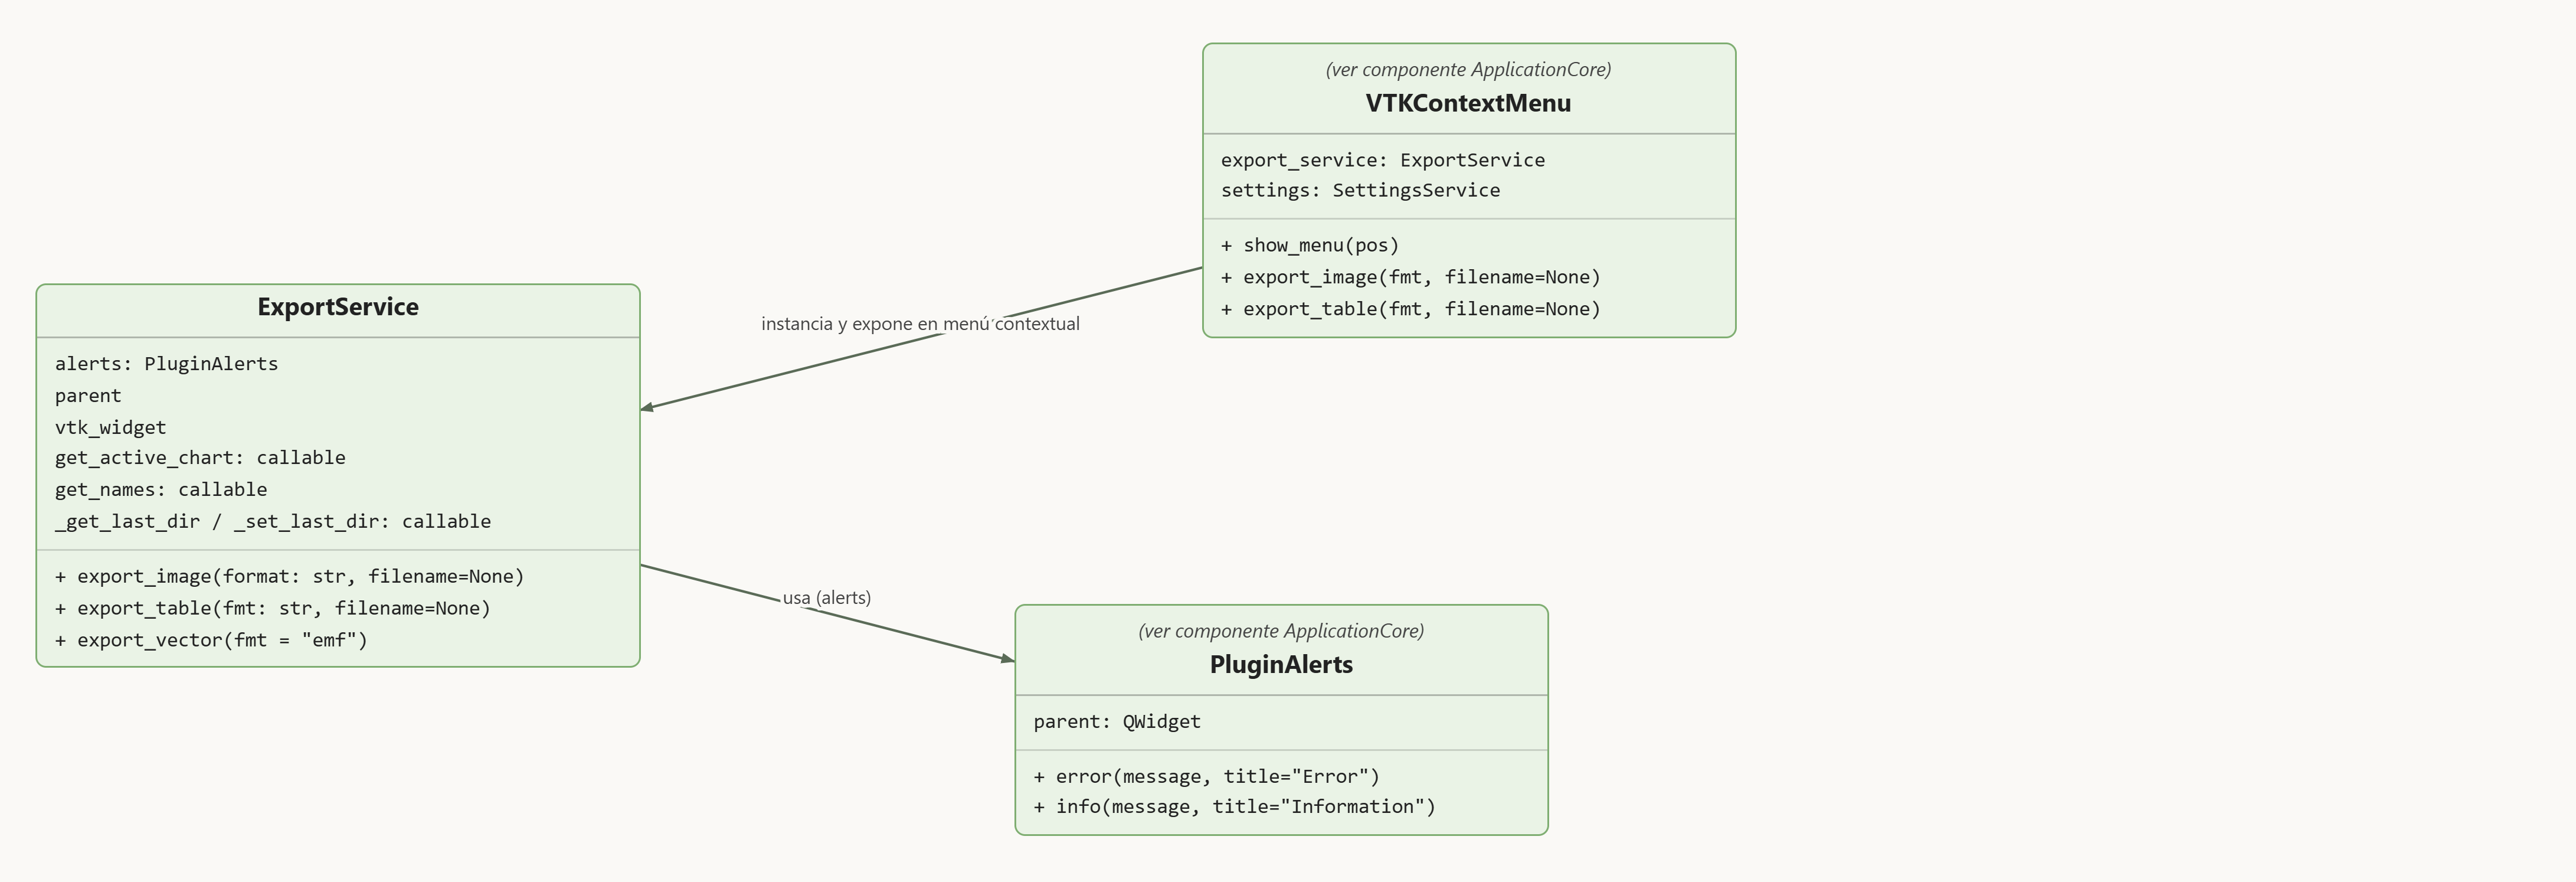
\includegraphics[width=0.85\linewidth]{diagramas_html/export.png}
    \caption{Diagrama de clases --- componente Export}
    \label{fig:sdd_dc_export}
\end{figure}

\textbf{ExportService} Servicio de exportación de imágenes y tablas a partir de la visualización VTK activa.
\begin{itemize}
    \item \textbf{Atributos principales:} \texttt{alerts: PluginAlerts}; \texttt{parent}; \texttt{vtk\_\allowbreak widget}; \texttt{get\_\allowbreak active\_\allowbreak chart}/\allowbreak\texttt{get\_\allowbreak names: callable}; \texttt{\_\allowbreak get\_\allowbreak last\_\allowbreak dir}/\allowbreak\texttt{\_\allowbreak set\_\allowbreak last\_\allowbreak dir: callable}.
    \item \textbf{Métodos principales:} \texttt{export\_\allowbreak image(format: str, filename=None)}, \texttt{export\_\allowbreak table(fmt: str, filename=None)}, \texttt{export\_\allowbreak vector(fmt = "emf")}.
\end{itemize}

\texttt{ExportService} no depende directamente de \texttt{VTKContextMenu}: recibe callbacks para desacoplarse de la interfaz que lo construye. Aun así, \texttt{VTKContextMenu} (ver componente ApplicationCore) sí lo instancia en su constructor y expone sus métodos en el menú contextual de cada gráfico; \texttt{ExportService} crea además su propia instancia de \texttt{PluginAlerts}. El SAD (Escenario de Calidad 4) describe a \texttt{ExportService} como registrado en el núcleo por inversión de control, pero \texttt{main.py} solo registra los servicios \texttt{"DataStore"} y \texttt{"FileIO"}: \texttt{ExportService} no está registrado en el Kernel, solo existe la instancia que crea \texttt{VTKContextMenu}. \texttt{export\_\allowbreak vector()} corresponde al caso de uso CU-017; no existe implementación de exportación vectorial (\texttt{.emf}) en el código --- solo están implementados \texttt{export\_\allowbreak image()} (png/jpg/jpeg/bmp/tiff) y \texttt{export\_\allowbreak table()} (csv/xlsx/json).

\item \textbf{Componente: Measurement}

El componente \textbf{Measurement} contiene la lógica para realizar mediciones interactivas de pendiente y amplitud sobre las señales.

\begin{figure}[htbp]
    \centering
    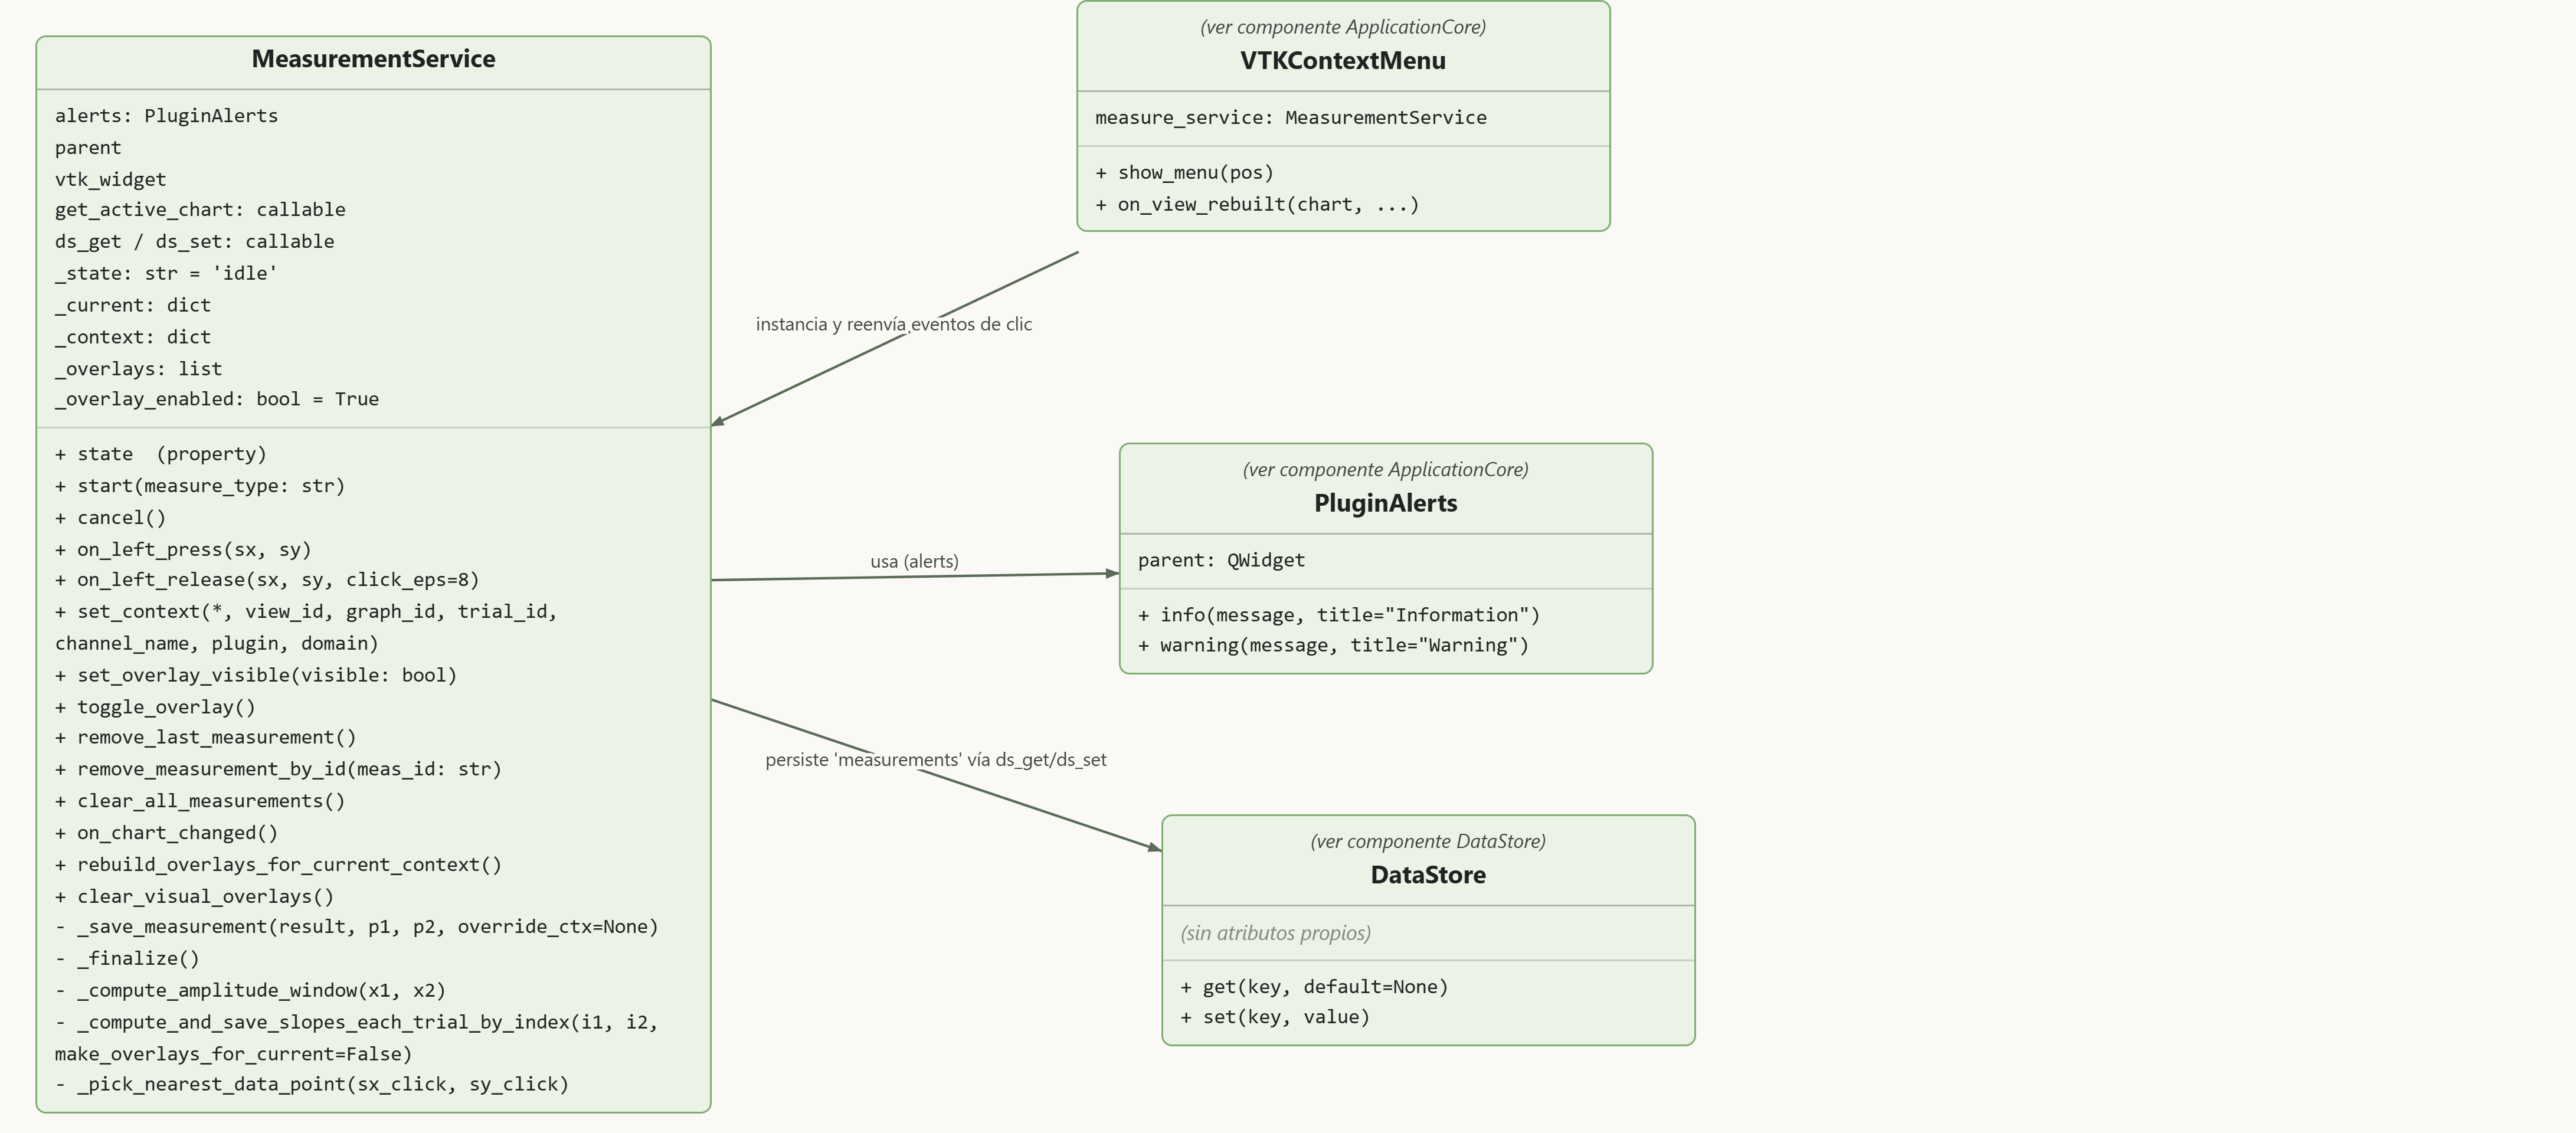
\includegraphics[width=0.95\linewidth]{diagramas_html/measurement.png}
    \caption{Diagrama de clases --- componente Measurement}
    \label{fig:sdd_dc_measurement}
\end{figure}

\textbf{MeasurementService} Servicio de medición que gestiona la selección de puntos, el cálculo y la persistencia de los resultados.
\begin{itemize}
    \item \textbf{Atributos principales:} \texttt{alerts: PluginAlerts}; \texttt{parent}; \texttt{vtk\_\allowbreak widget}; \texttt{get\_\allowbreak active\_\allowbreak chart: callable}; \texttt{ds\_\allowbreak get}/\allowbreak\texttt{ds\_\allowbreak set: callable}; \texttt{\_\allowbreak state: str = 'idle'}; \texttt{\_\allowbreak current: dict}; \texttt{\_\allowbreak context: dict}; \texttt{\_\allowbreak overlays: list}; \texttt{\_\allowbreak overlay\_\allowbreak enabled: bool = True}.
    \item \textbf{Métodos principales:} \texttt{state} (propiedad), \texttt{start(measure\_\allowbreak type: str)}, \texttt{cancel()}, \texttt{on\_\allowbreak left\_\allowbreak press(sx, sy)}, \texttt{on\_\allowbreak left\_\allowbreak release(sx, sy, click\_\allowbreak eps=8)}, \texttt{set\_\allowbreak context(\ldots)}, \texttt{set\_\allowbreak overlay\_\allowbreak visible(visible: bool)}, \texttt{toggle\_\allowbreak overlay()}, \texttt{remove\_\allowbreak last\_\allowbreak measurement()}, \texttt{remove\_\allowbreak measurement\_\allowbreak by\_\allowbreak id(meas\_\allowbreak id: str)}, \texttt{clear\_\allowbreak all\_\allowbreak measurements()}, \texttt{on\_\allowbreak chart\_\allowbreak changed()}, \texttt{rebuild\_\allowbreak overlays\_\allowbreak for\_\allowbreak current\_\allowbreak context()}, \texttt{clear\_\allowbreak visual\_\allowbreak overlays()}.
\end{itemize}

\texttt{VTKContextMenu} (ver componente ApplicationCore) instancia \texttt{MeasurementService} en su constructor y le reenvía los eventos de clic izquierdo del \texttt{vtk\_\allowbreak widget}. Los resultados se persisten en \texttt{DataStore} bajo la clave \texttt{"measurements"} --- la misma instancia que ya almacena señales y trials --- mediante los callbacks \texttt{ds\_\allowbreak get}/\allowbreak\texttt{ds\_\allowbreak set}. \texttt{MeasurementService} crea su propia instancia de \texttt{PluginAlerts} y usa \texttt{two\_\allowbreak point\_\allowbreak metrics()}/\allowbreak\texttt{amplitude\_\allowbreak in\_\allowbreak window()} de \texttt{core/filters/measurements.py} para el cálculo numérico. Al igual que \texttt{ExportService}, no está registrado como servicio del Kernel pese a que el SAD lo describe así: solo existe la instancia que crea \texttt{VTKContextMenu}.

\item \textbf{Componente: ProjectSession} (nuevo, sin equivalente en GammaLab 1.0)

El componente \textbf{ProjectSession} materializa el atributo de calidad "Trazabilidad y Persistencia" que GammaLab 2.0 introduce: la persistencia local del espacio de trabajo completo en archivos de proyecto \texttt{.glab}.

\begin{figure}[htbp]
    \centering
    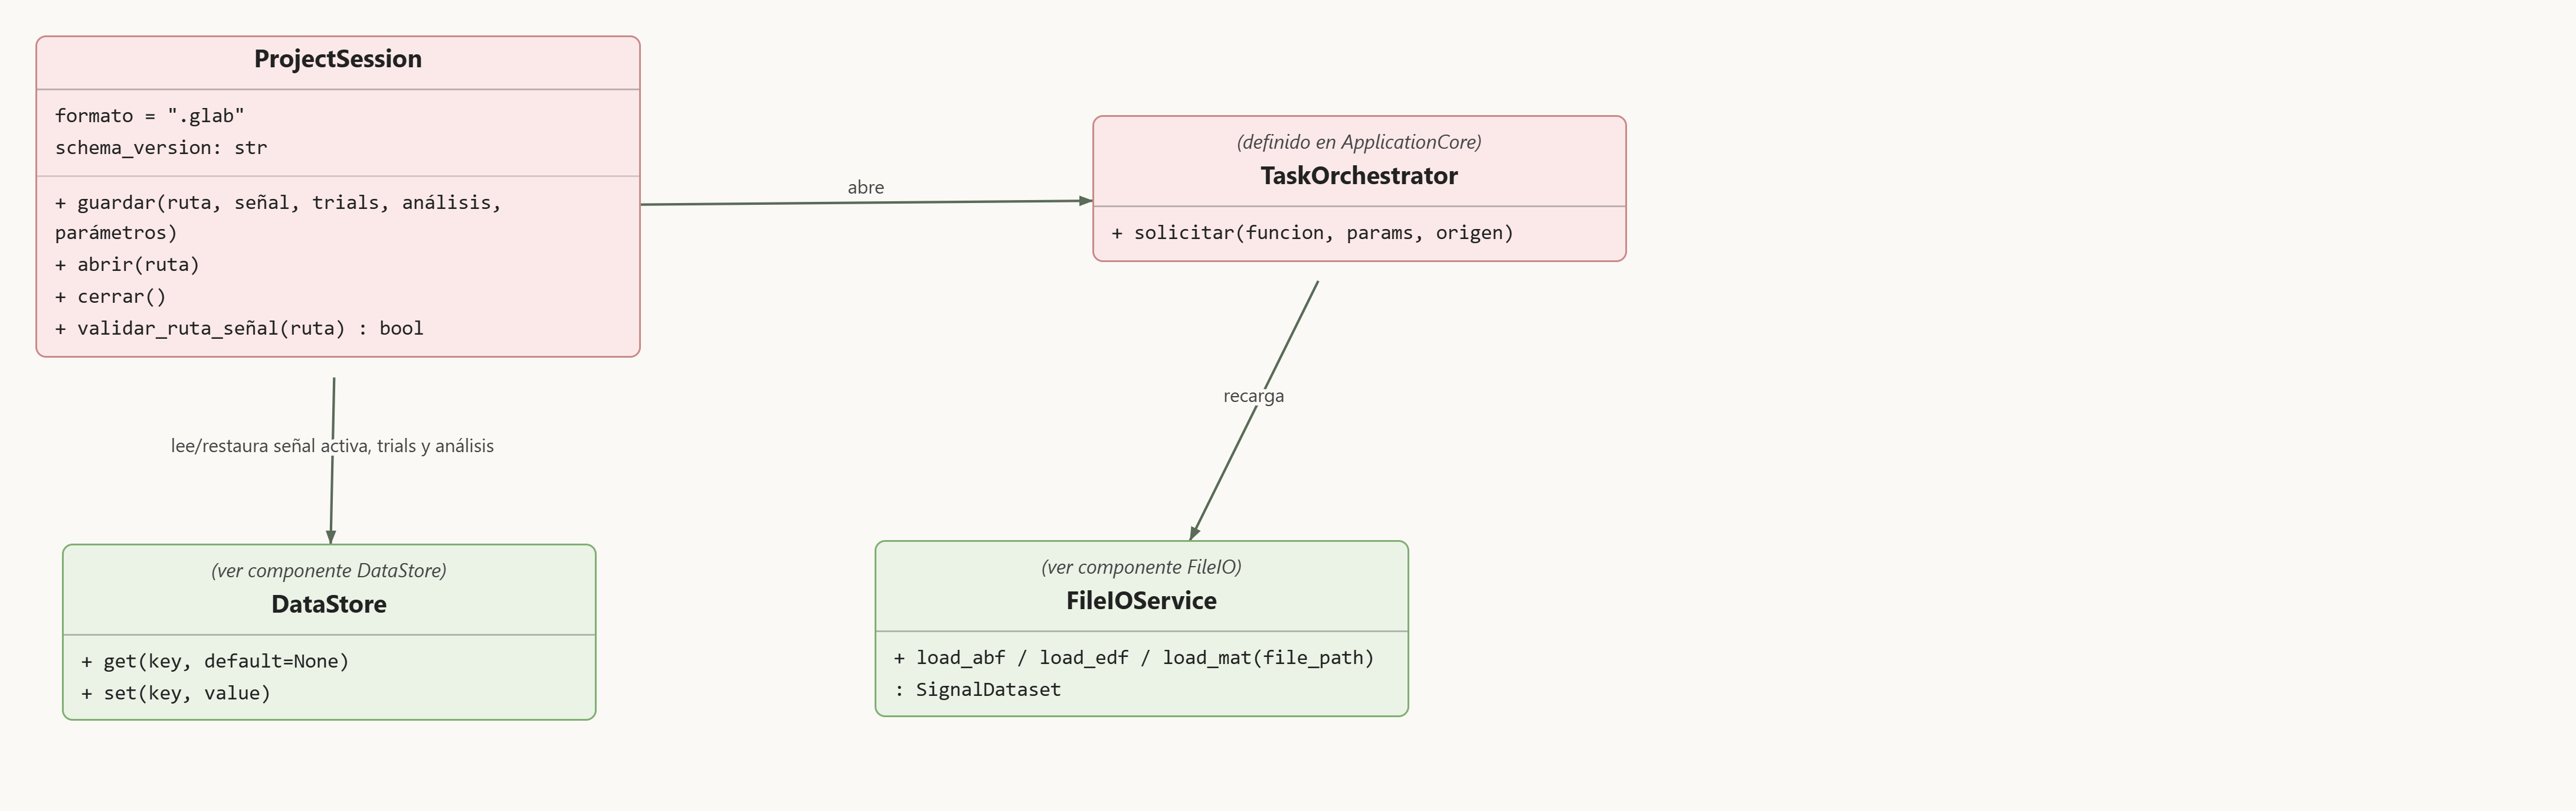
\includegraphics[width=0.85\linewidth]{diagramas_html/project_session.png}
    \caption{Diagrama de clases --- componente ProjectSession}
    \label{fig:sdd_dc_projectsession}
\end{figure}

\textbf{ProjectSession} (nuevo) Gestiona la persistencia del espacio de trabajo en archivos \texttt{.glab}.
\begin{itemize}
    \item \textbf{Atributos principales:} \texttt{formato = ".glab"}; \texttt{schema\_\allowbreak version: str}.
    \item \textbf{Métodos principales:} \texttt{guardar(ruta, señal, trials, análisis, parámetros)}, \texttt{abrir(ruta)}, \texttt{cerrar()}, \texttt{validar\_\allowbreak ruta\_\allowbreak señal(ruta): bool}.
\end{itemize}

Ninguna clase de este componente existe hoy en el código --- hay cero referencias a \texttt{".glab"} en todo el repositorio (SAD, UC-03) --- pero sus relaciones sí se apoyan en clases reales: \texttt{guardar()} persiste señal, trials, análisis y parámetros en el \texttt{.glab} y libera la memoria de la señal activa; \texttt{abrir(ruta)} verifica con \texttt{validar\_\allowbreak ruta\_\allowbreak señal()} que el archivo de señal referenciado siga disponible y despacha su recarga al \texttt{TaskOrchestrator} fuera del hilo de interfaz, que a su vez reutilizaría \texttt{FileIOService} (ver componente FileIO); los trials y análisis se restauran directamente en \texttt{DataStore} mediante escritura sincronizada. Cada \texttt{.glab} embebe su propio \texttt{schema\_\allowbreak version}: un incremento MINOR se mantiene legible por versiones futuras de \texttt{ProjectSession}, y un incremento MAJOR rechaza la apertura con un mensaje explícito en vez de migrar implícitamente.

\end{enumerate}

\subsubsection{Resumen}

\begin{itemize}
    \item \textbf{Patrón arquitectónico:} inversión de control mediante el \texttt{Kernel}, que expone \texttt{register\_\allowbreak service()}/\allowbreak\texttt{get\_\allowbreak service()} y desacopla a los plugins de la construcción directa de sus dependencias.
    \item \textbf{Relación central:} todos los plugins concretos implementan \texttt{IPlugin} y son descubiertos y gestionados por \texttt{PluginManager}/\allowbreak\texttt{Kernel} a partir de su \texttt{properties.yml}.
    \item \textbf{Servicios resueltos vía Kernel:} \texttt{DataStore} y \texttt{FileIOService} (bajo la clave \texttt{"FileIO"}) sí se consumen mediante \texttt{kernel.get\_\allowbreak service()}.
    \item \textbf{Servicios instanciados directamente:} \texttt{ExportService} y \texttt{MeasurementService} son construidos directamente por \texttt{VTKContextMenu}, y \texttt{SettingsService} no se registra en \texttt{main.py}; los tres aparecen en el SAD como servicios del núcleo, pero ninguno se resuelve hoy mediante \texttt{kernel.get\_\allowbreak service()}.
    \item \textbf{Piezas prospectivas:} \texttt{TaskOrchestrator}, \texttt{ProjectSession}, \texttt{TooltipHelper} y la familia \texttt{PACAnalysisPlugin} no existen aún en el código; el SAD los presenta como criterios de aceptación directos para la implementación futura, no como documentación de un sistema ya construido.
    \item \textbf{Flujo de control:} \texttt{MainWindow} actúa como contenedor principal que orquesta la interacción entre plugins a través del \texttt{Kernel}.
\end{itemize}

\subsection{Comportamiento del Sistema}

\subsubsection{Propósito}

El objetivo de esta sección es documentar los flujos más importantes del sistema a nivel de interacción entre objetos, complementando la Vista de Procesos (Sección 2.3), que describe el mismo comportamiento a nivel de actividades del usuario.

\subsubsection{Principales flujos del sistema}

Los flujos descritos abarcan cuatro funcionalidades: la carga de una señal, la toma de mediciones, la exportación de resultados y --- como flujo prospectivo, aún no implementado --- el guardado y reapertura de un proyecto.

\textbf{1. Cargar una señal.} Desde la pestaña \textit{Home}, el usuario activa \textit{Load Signal}; \texttt{OpenSignalPlugin} obtiene el servicio \texttt{FileIOService} del Kernel (clave \texttt{"FileIO"}) o crea una instancia propia si no lo encuentra registrado. Según la extensión del archivo, invoca \texttt{load\_\allowbreak abf()} o \texttt{load\_\allowbreak edf()} de forma directa y síncrona sobre el hilo de interfaz --- la rama de \texttt{load\_\allowbreak mat()} existe en \texttt{FileIOService} pero está comentada en el plugin. El resultado, una instancia de \texttt{SignalDataset}, se publica en \texttt{DataStore} como señal activa y \texttt{MainWindow} actualiza la lista de señales disponibles.

\textbf{2. Hacer mediciones.} El usuario hace clic derecho sobre un gráfico, lo que activa \texttt{VTKContextMenu.show\_\allowbreak menu()} y despliega el menú contextual con las opciones \textit{Slope}, \textit{Amplitude} y \textit{Slope (all trials)}. Al seleccionar una, se invoca \texttt{MeasurementService.start(measure\_\allowbreak type)}, que usa \texttt{PluginAlerts} para solicitar al usuario los dos puntos requeridos. Cada clic del usuario se recibe mediante \texttt{on\_\allowbreak left\_\allowbreak press()}/\allowbreak\texttt{on\_\allowbreak left\_\allowbreak release()}; una vez capturados ambos puntos, \texttt{\_\allowbreak finalize()} calcula el resultado con \texttt{two\_\allowbreak point\_\allowbreak metrics()} (pendiente) o \texttt{amplitude\_\allowbreak in\_\allowbreak window()} (amplitud) de \texttt{core/filters/measurements.py}, dibuja el overlay correspondiente y persiste el registro en \texttt{DataStore} bajo la clave \texttt{"measurements"} mediante \texttt{\_\allowbreak save\_\allowbreak measurement()}.

\textbf{3. Exportar resultados.} El usuario hace clic derecho sobre un gráfico y selecciona \textit{Export as image} o \textit{Export table} desde el menú de \texttt{VTKContextMenu}. Según la opción, se invoca \texttt{ExportService.export\_\allowbreak image(format)} --- que captura la ventana VTK con \texttt{vtkWindowToImageFilter} y la escribe con el \textit{writer} correspondiente a png/jpg/jpeg/bmp/tiff --- o \texttt{export\_\allowbreak table(fmt)}, que recorre los \textit{plots} del gráfico activo y escribe el resultado en csv, xlsx o json. En ambos casos, \texttt{ExportService} usa \texttt{PluginAlerts} para confirmar el éxito o reportar un error, sin interrumpir el estado del sistema.

\textbf{4. Guardar y reabrir un proyecto (prospectivo).} Al cerrar el proyecto activo, el investigador elige \textit{Guardar}; \texttt{ProjectSession.guardar()} persistiría la señal activa, los trials, los análisis y los parámetros de la sesión en un archivo \texttt{.glab}, liberando a continuación la memoria de la señal activa. Al abrir un \texttt{.glab} existente, \texttt{abrir(ruta)} verificaría con \texttt{validar\_\allowbreak ruta\_\allowbreak señal()} que el archivo de señal referenciado siga disponible, despacharía su recarga al \texttt{TaskOrchestrator} --- que reutilizaría \texttt{FileIOService} fuera del hilo de interfaz --- y restauraría los trials y análisis directamente en \texttt{DataStore} mediante escritura sincronizada. Ninguna clase de este flujo existe hoy en el código: es el criterio de aceptación para la funcionalidad descrita en el SAD (UC-03).

\subsection{Persistencia y Modelos de Datos}

\subsubsection{Propósito}

El objetivo de esta sección es describir las estructuras en las que se almacenan los datos de la aplicación y los mecanismos de persistencia que permiten el funcionamiento de los plugins. El sistema no emplea bases de datos: la persistencia es temporal y está basada en un almacén clave-valor en memoria (\texttt{DataStore}), accedido a través de sus métodos \texttt{get}/\allowbreak\texttt{set}.

\subsubsection{Entidades de datos}

El diagrama de clases del componente DataStore, ya presentado en la Figura~\ref{fig:sdd_dc_datastore} (Sección 3.2.3), ilustra las tres entidades centrales del modelo de datos: \texttt{DataStore}, \texttt{SignalDataset} y \texttt{TrialDataset}.

\textbf{DataStore} Servicio central de almacenamiento; mantiene un diccionario interno (\texttt{\_\allowbreak data}) indexado por clave, sin imponer un esquema fijo. Sus usos principales son:
\begin{itemize}
    \item Ciclo de vida de las señales cargadas: \texttt{add\_\allowbreak signal()}, \texttt{get\_\allowbreak signals()}, \texttt{set\_\allowbreak active\_\allowbreak signal()}/\allowbreak\texttt{get\_\allowbreak active\_\allowbreak signal()}.
    \item Almacenamiento genérico de cualquier otro estado bajo una clave arbitraria mediante \texttt{set(key, value)}/\allowbreak\texttt{get(key, default)}: además de señales, \texttt{MeasurementService} (ver componente Measurement) lo reutiliza para persistir las mediciones bajo la clave \texttt{"measurements"}, sin que \texttt{DataStore} distinga entre ambos tipos de contenido.
\end{itemize}

\textbf{SignalDataset} Representa una señal completa cargada por \texttt{FileIOService} (ver componente FileIO): incluye los arreglos de tiempo y de señal, los metadatos de canal y muestreo, y la lista de \texttt{TrialDataset} asociados a ella.

\textbf{TrialDataset} Representa un ensayo (segmento) de una señal, con su propia base de tiempo relativa, sus marcadores de \textit{onset} e \textit{ISI}, y sus metadatos de canal y fuente. No tiene métodos propios: es una estructura de datos consumida por \texttt{SignalDataset}.

\subsection{Relaciones}

La relación principal del modelo de datos es la que existe entre \texttt{SignalDataset} y \texttt{TrialDataset}: la multiplicidad 1 a muchos (1..*) indica que una señal puede contener múltiples trials, cada uno representando un segmento de interés para el análisis. Esta relación se mantiene igual que en GammaLab 1.0.

Sobre esa base, GammaLab 2.0 generaliza el uso de \texttt{DataStore} más allá de señales y trials: al ser un almacén clave-valor sin esquema fijo, la misma instancia registrada en el Kernel también persiste las mediciones de \texttt{MeasurementService} (clave \texttt{"measurements"}), y sería el punto de lectura/escritura de \texttt{TaskOrchestrator} y \texttt{ProjectSession} una vez implementados.

Un segundo patrón de relación distingue a los componentes según cómo se resuelven sus dependencias: \texttt{DataStore} y \texttt{FileIOService} se consumen mediante \texttt{kernel.get\_\allowbreak service()}, mientras que \texttt{ExportService} y \texttt{MeasurementService} se obtienen por inyección directa desde \texttt{VTKContextMenu} en su constructor, sin pasar por el Kernel. Ambos patrones conviven hoy en el sistema, aunque el SAD describe a los cinco servicios como igualmente registrados en el núcleo.

\subsection{Interfaz de Usuario}
         \subsubsection{Proposito}
            Esta sección describe la interfaz de usuario de Gamma Lab, incluyendo la organización, navegación, y componentes de las vistas.

        \subsubsection{Organización de la pantalla principal}
        \begin{figure}[H]
            \centering
            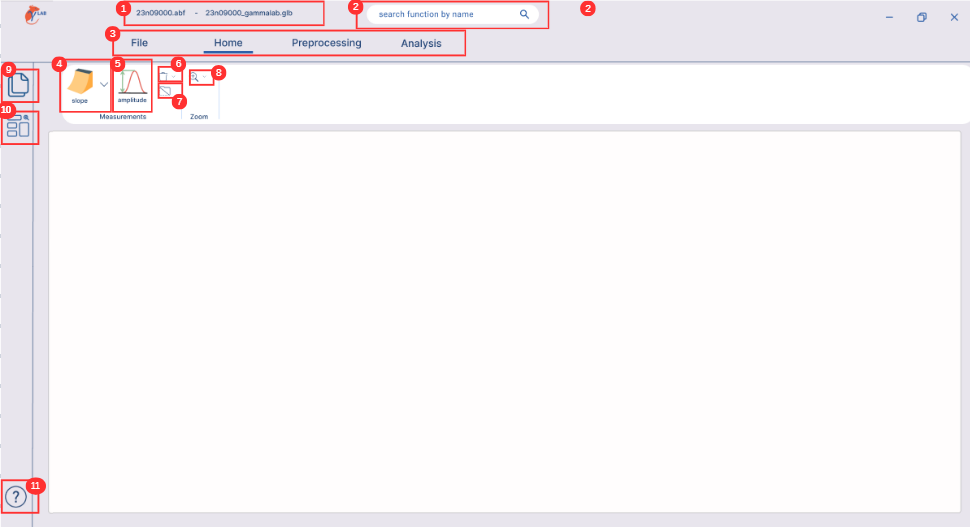
\includegraphics[width=0.8\textwidth]{home.png}
            \caption{Organización de la pantalla principal de Gamma Lab}
            \label{fig:interfaz_principal}
        \end{figure}

        La pantalla principal se compone de los siguientes elementos, numerados en la Figura \ref{fig:interfaz_principal}:
        \begin{itemize}
            \item \textbf{1 - Panel de control:} muestra el nombre de la señal abierta junto al nombre, editable, del proyecto activo, guardado con extensión \texttt{.glab}.
            \item \textbf{2 - Barra de búsqueda:} ubicada en la parte superior, permite localizar y acceder rápidamente a una funcionalidad específica del sistema sin tener que recorrer manualmente la barra de navegación.
            \item \textbf{3 - Barra de navegación:} agrupa las pestañas \textit{File}, \textit{Home}, \textit{Preprocessing} y \textit{Analysis}, permitiendo alternar entre la gestión de archivos, las mediciones sobre la señal, el preprocesamiento y los módulos de análisis.
            \item \textbf{4 - slope:} opción de la categoría \textit{Measurements} (pestaña \textit{Home}) que permite medir la pendiente de la señal entre dos puntos seleccionados por el usuario, mediante las subopciones \textit{Slope 2 Trials} (calculada sobre dos ensayos) y \textit{Slope All Trials} (calculada sobre la totalidad de los ensayos generados).
                    \begin{figure}[H]
                     \centering
                     
\includegraphics[width=0.5\textwidth]{slope.png}
                        \caption{opciones de slope}
                        \label{fig:slope}
                    \end{figure}
            \item \textbf{5 - amplitude:} opción de la categoría \textit{Measurements} (pestaña \textit{Home}) que permite medir la amplitud de la señal entre dos puntos seleccionados por el usuario sobre la gráfica.
            \item \textbf{6 - eliminar medida:} permite eliminar la última medición de \textit{slope} o \textit{amplitude} realizada, o bien la totalidad de las mediciones registradas sobre la señal.
                    \begin{figure}[H]
                     \centering
                     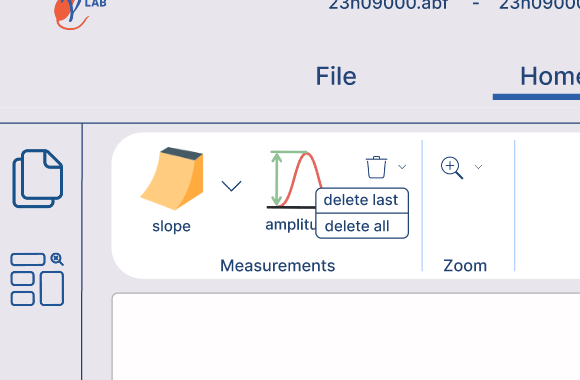
\includegraphics[width=0.5\textwidth]{eliminar.png}
                        \caption{opciones de eliminar medida}
                        \label{fig:eliminarMedida}
                    \end{figure}
            \item \textbf{7 - mostrar/ocultar:} permite mostrar u ocultar en pantalla las mediciones de \textit{slope} y \textit{amplitude} realizadas previamente sobre la señal, sin necesidad de eliminarlas.
            \item \textbf{8 - zoom:} activa o desactiva la función de acercamiento sobre la gráfica de la señal, permitiendo observar con mayor detalle un segmento de la señal y las mediciones realizadas sobre él.
                \begin{figure}[H]
                     \centering
                     
\includegraphics[width=0.5\textwidth]{zoom.png}
                        \caption{opciones de zoom}
                        \label{fig:zoom}
                \end{figure}
            \item \textbf{9 - explorador de archivos:} despliega, desde la barra lateral izquierda, la carpeta del sistema de archivos en la que se encuentra almacenado el proyecto actual junto con las señales y resultados exportados, sin salir de la aplicación.
                    \begin{figure}[H]
                     \centering
                     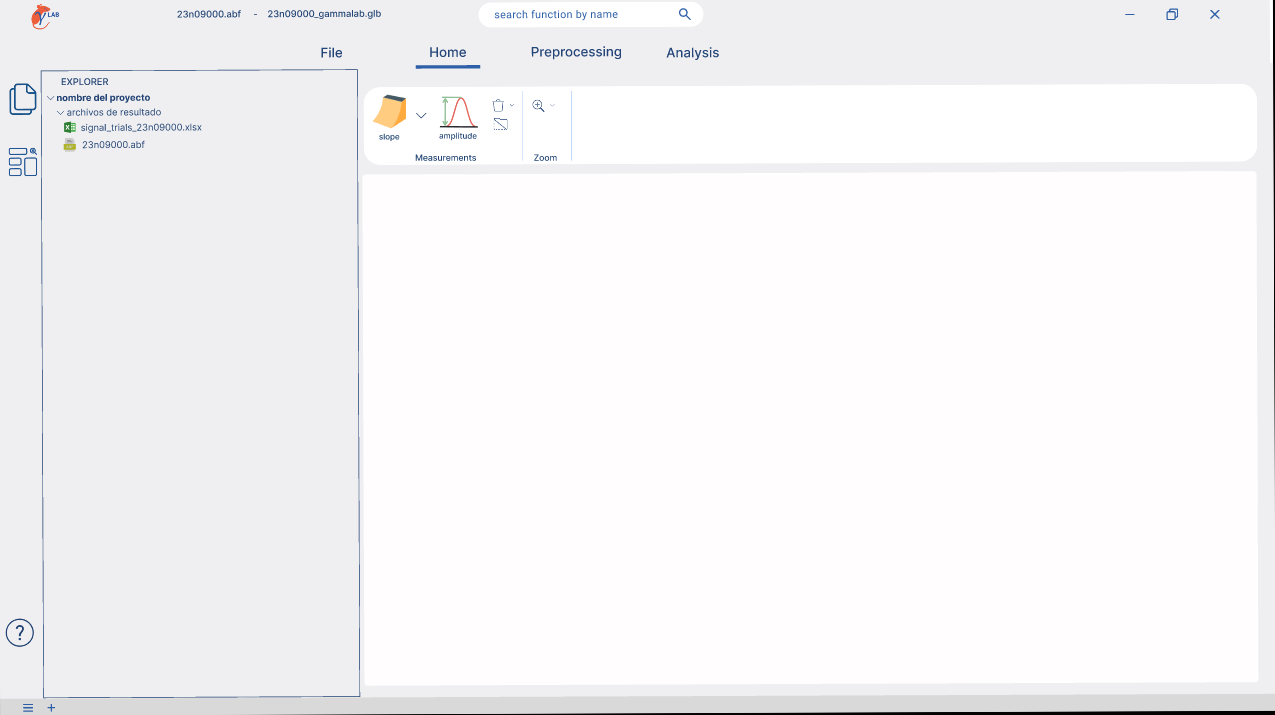
\includegraphics[width=0.5\textwidth]{exploradorArchivos.png}
                        \caption{explorador de archivos desplegado}
                        \label{fig:explorador}
                    \end{figure}
            \item \textbf{10 - resultados:} despliega, desde la barra lateral izquierda, una ventana inferior con los resultados numéricos de las mediciones de \textit{slope} y \textit{amplitude} realizadas sobre la señal, los cuales pueden exportarse en formato \texttt{.csv} para su análisis externo.
                    \begin{figure}[H]
                     \centering
                     
\includegraphics[width=0.5\textwidth]{resultados.png}
                        \caption{resultados desplegados}
                        \label{fig:resultados}
                    \end{figure}
                    \begin{figure}[H]
                        \centering
                        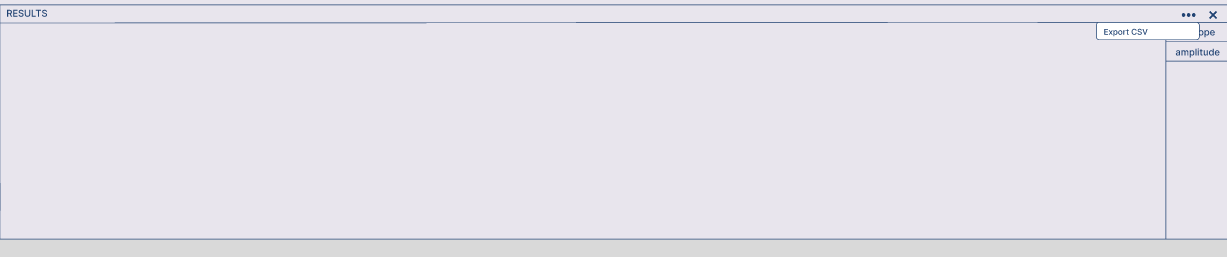
\includegraphics[width=0.5\textwidth]{resultados2.png}
                        \caption{Los resultados pueden ser exportados en formato csv.}
                        \label{fig:resultados2}
                    \end{figure}
            \item \textbf{11 - ayuda:} despliega, desde la barra lateral izquierda, el manual de usuario del sistema, con información de referencia sobre el uso de cada funcionalidad.
        \end{itemize}

        \subsubsection{Carga y guardado de archivos (pestaña \textit{File})}

        \begin{figure}[H]
            \centering
            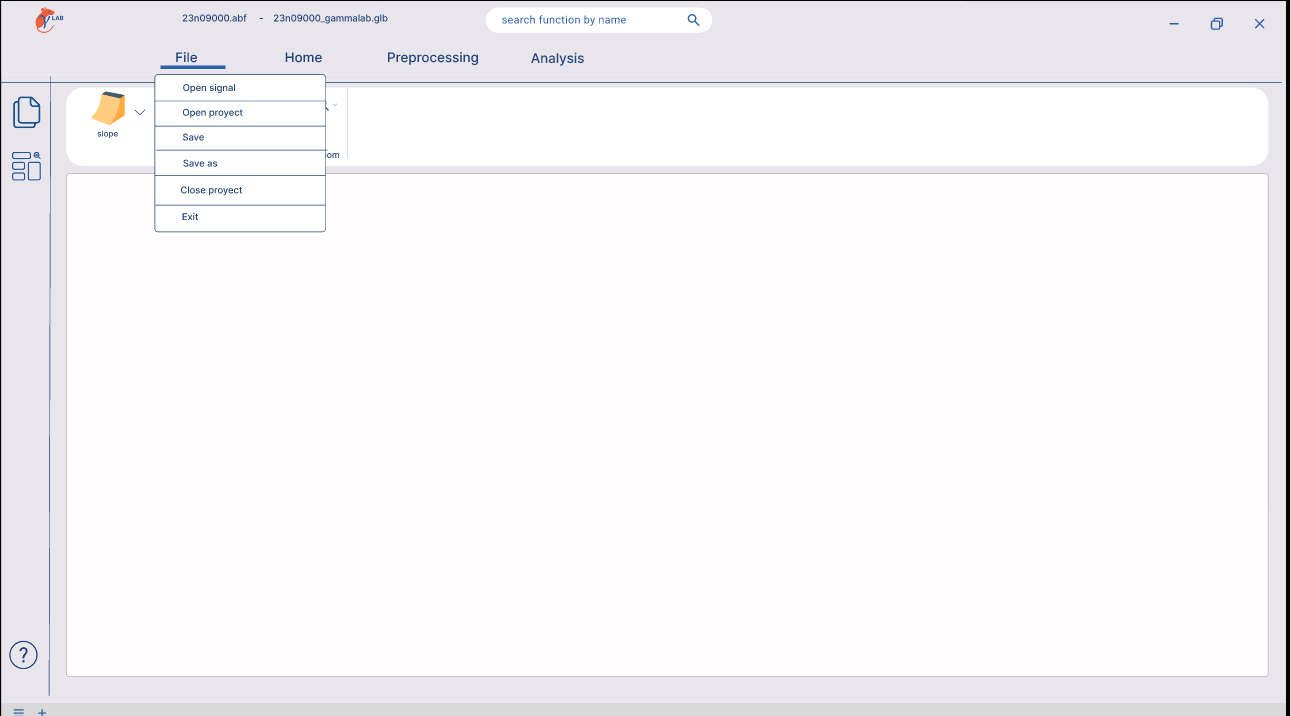
\includegraphics[width=0.8\textwidth]{file.png}
            \caption{Pestaña File de Gamma Lab}
            \label{fig:file_tab}
        \end{figure}

        La pestaña \textit{File} permite gestionar la carga y el guardado de señales y proyectos. Agrupa las siguientes opciones:

        \begin{itemize}
            \item \textbf{Open Signal:} permite cargar una señal individual dentro de la aplicación para su preprocesamiento y análisis.
            \item \textbf{Open Project:} permite abrir un proyecto previamente guardado con extensión \texttt{.glab}, restaurando la señal activa, los trials, los análisis y los parámetros de la sesión.
            \item \textbf{Save:} guarda los cambios realizados sobre el proyecto actualmente abierto.
            \item \textbf{Save As:} permite guardar el proyecto actual bajo un nuevo nombre o ubicación, sin sobrescribir el archivo original.
            \item \textbf{Close Project:} cierra el proyecto que se encuentra abierto, liberando la señal activa de memoria.
            \item \textbf{Exit:} cierra la aplicación.
        \end{itemize}

        A continuación se ilustra el flujo de carga de una señal y de un proyecto:

       \begin{figure}[H]
            \centering
            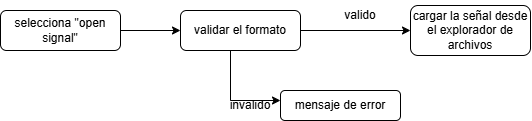
\includegraphics[width=0.8\textwidth]{cargarSeñal.png}
            \caption{Flujo de carga de la señal (\textit{Open Signal})}
            \label{fig:cargar_senal}
        \end{figure}

        \begin{figure}[H]
            \centering
            \includegraphics[width=0.8\textwidth]{cargarproyecto.png}
            \caption{Flujo de carga de proyecto (\textit{Open Project})}
            \label{fig:cargar_proyecto}
        \end{figure}

        Mediante las opciones \textit{Save} y \textit{Save As} es posible almacenar el estado completo del espacio de trabajo, incluyendo la señal activa, los trials configurados, las medidas realizadas y los resultados de los análisis ejecutados, en un archivo de proyecto con extensión \texttt{.glab}.

        \subsubsection{Preprocesamiento}

        \begin{figure}[H]
            \centering
            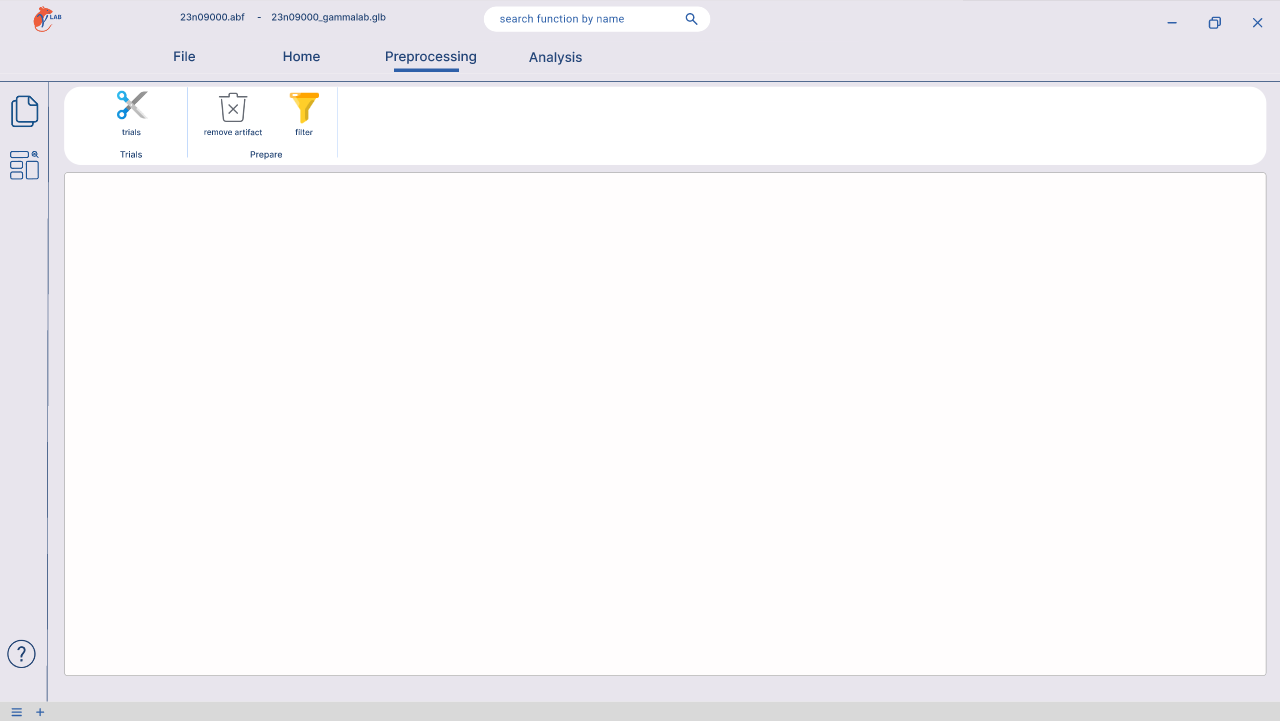
\includegraphics[width=0.8\textwidth]{preprocessing.png}
            \caption{Pestaña Preprocessing de Gamma Lab}
            \label{fig:preprocessing_tab}
        \end{figure}

        \textbf{Categoria \textit{Trials}}
        \begin{itemize}
            \item \textbf{trials:} divide la señal cargada en ensayos (\textit{trials}), permitiendo seleccionar el canal a dividir, el canal de estímulos, el umbral (\textit{threshold}), el número de estímulos y el tamaño de la ventana de segmentación. Una vez generados, el usuario puede navegar entre los trials resultantes e incluirlos o descartarlos individualmente del conjunto que participará en los análisis posteriores.
            \begin{figure}[H]
                \centering
                
\includegraphics[width=0.8\textwidth]{trials.png}
                \caption{opciones de trials}
                \label{fig:trials}
            \end{figure}
        \end{itemize}

        \textbf{Categoria \textit{prepare}}
        \begin{itemize}
            \item \textbf{remove artifact:} elimina artefactos presentes en los trials mediante la selección de un rango de tiempo a corregir, ofreciendo dos modos de corrección: interpolación del segmento seleccionado o eliminación de la señal desde el inicio del trial hasta el punto seleccionado.
            \begin{figure}[H]
                \centering
                \includegraphics[width=0.8\textwidth]{removeartifact.png}
                \caption{opciones de remove artifact}
                \label{fig:removeartifact}
            \end{figure}
            \item \textbf{filter:} aplica un filtro digital Butterworth a la señal, mediante la selección del rango de frecuencias de corte y el orden del filtro, mostrando el resultado tanto sobre la señal completa como sobre el primer trial generado.
            \begin{figure}[H]
                \centering
                
\includegraphics[width=0.8\textwidth]{filter.png}
                \caption{opciones de filter}
                \label{fig:filter}
            \end{figure}
        \end{itemize}
    
    \subsubsection{Analysis}
    En esta sección se pueden realizar diferentes análisis de la señal, a continuación seran listados los análisis disponibles y sus opciones:

    \begin{itemize}
        \item \textbf{FFT: } calcula la transformada rápida de Fourier de la señal, mediante la configuración de la frecuencia de muestreo y el rango de frecuencias de interés, y muestra el espectro de potencia resultante de forma individual para cada ensayo.
            \begin{figure}[H]
                \centering
                \includegraphics[width=0.8\textwidth]{fft.png}
                \caption{opciones de FFT}
                \label{fig:fft}
            \end{figure}
        \item \textbf{FFT Average:} calcula la FFT de la señal con la misma configuración de frecuencia de muestreo y rango de frecuencias que la opción anterior, pero adicionalmente promedia los espectros obtenidos de todos los ensayos para reducir el ruido y resaltar los componentes de frecuencia comunes entre ellos.
            \begin{figure}[H]
                \centering
                \includegraphics[width=0.8\textwidth]{fftaverage.png}
                \caption{opciones de FFT Average}
                \label{fig:fftaverage}
            \end{figure}
        \item \textbf{PSD: } estima la densidad espectral de potencia de la señal mediante el método de Welch, permitiendo configurar el modo de cálculo, el tipo de ventana, el rango de frecuencias y el modo de \textit{detrend}, y muestra el resultado de forma individual para cada ensayo.
            \begin{figure}[H]
                \centering
                \includegraphics[width=0.8\textwidth]{psd.png}
                \caption{opciones de PSD}
                \label{fig:psd}
            \end{figure}
        \item \textbf{PSD Average:} estima la PSD de la señal mediante el método de Welch, con la misma configuración de frecuencia de muestreo, ventana y rango de frecuencias que la opción anterior, pero promediando de forma agregada los resultados de todos los ensayos.
            \begin{figure}[H]
                \centering
                \includegraphics[width=0.8\textwidth]{psdaverage.png}
                \caption{opciones de PSD Average}
                \label{fig:psdaverage}
            \end{figure}
        \item \textbf{PSD relative: } calcula la PSD relativa de la señal, entregando tanto la potencia absoluta como la potencia relativa aportada por cada banda de frecuencia del rango seleccionado, mediante la configuración del tipo de ventana, el modo de \textit{detrend} y el modo de cálculo.

        \item \textbf{Average: } calcula y visualiza el promedio temporal de los trials generados, útil para observar patrones comunes y atenuar variaciones aleatorias entre ensayos.
            \begin{figure}[H]
                \centering
                
\includegraphics[width=0.8\textwidth]{average.png}
                \caption{opciones de Average}
                \label{fig:average}
            \end{figure}
        \item \textbf{Event related potential: } calcula el potencial relacionado con eventos (ERP), generando un \textit{Butterfly Plot} con todos los trials alineados y un espectrograma de la dinámica tiempo-frecuencia asociada al evento.
            \begin{figure}[H]
                \centering
                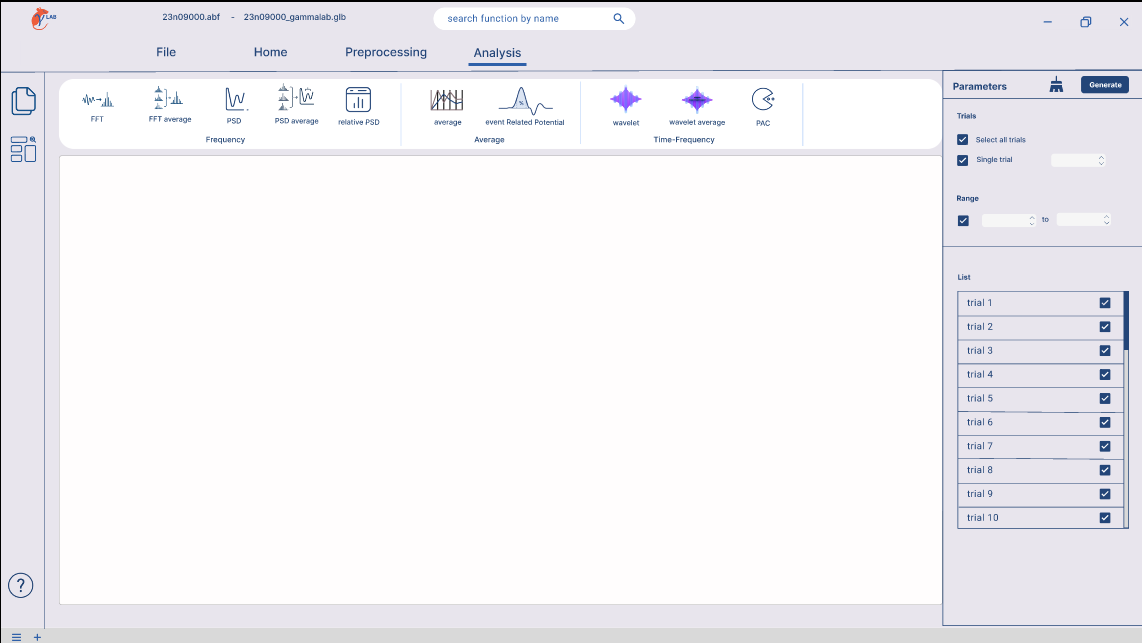
\includegraphics[width=0.8\textwidth]{eventRelated.png}
                \caption{opciones de Event related potential}
                \label{fig:erp}
            \end{figure}
        \item \textbf{Wavelet: } calcula la transformada wavelet continua de la señal, mediante la configuración de la frecuencia de muestreo, el rango de frecuencias, el número de ciclos, la normalización y la escala de visualización, permitiendo observar cómo varía el contenido espectral de la señal a lo largo del tiempo para cada ensayo.
            \begin{figure}[H]
                \centering
                
\includegraphics[width=0.8\textwidth]{wavelet.png}
                \caption{opciones de Wavelet}
                \label{fig:wavelet}
            \end{figure}
        \item \textbf{Wavelet Average: } calcula la transformada wavelet con la misma configuración que la opción anterior, y promedia los resultados sobre múltiples trials, generando un mapa tiempo-frecuencia agrupado.
            \begin{figure}[H]
                \centering
                \includegraphics[width=0.8\textwidth]{waveletaverage.png}
                \caption{opciones de Wavelet Average}
                \label{fig:waveletaverage}
            \end{figure}
        \item \textbf{PAC: } calcula el acoplamiento de fase-amplitud (\textit{Phase-Amplitude Coupling}) de un canal, evaluando la relación entre la fase de una banda de baja frecuencia y la amplitud de un rango de frecuencias seleccionado, ya sea sobre un trial individual o sobre el promedio de varios trials. El resultado incluye el mapa de acoplamiento fase-frecuencia, el histograma de distribución de amplitud en función de la fase, y el vector de acoplamiento medio con su magnitud y ángulo.
            \begin{figure}[H]
                \centering
                \includegraphics[width=0.8\textwidth]{pac.png}
                \caption{opciones de PAC}
                \label{fig:pac}
            \end{figure}
    \end{itemize}

\end{document}